% !TEX root = ../main.tex
\documentclass{report}


%%%%%%%%%%%%%%%%%%%%%%%%%%%%%%%%%
% PACKAGE IMPORTS
%%%%%%%%%%%%%%%%%%%%%%%%%%%%%%%%%


\usepackage[tmargin=2cm,rmargin=1in,lmargin=1in,margin=0.85in,bmargin=2cm,footskip=.2in]{geometry}
\usepackage{amsmath,amsfonts,amsthm,amssymb,mathtools}
\usepackage[varbb]{newpxmath}
\usepackage{xfrac}
\usepackage[makeroom]{cancel}
\usepackage{mathtools}
\usepackage{bookmark}
\usepackage{enumitem}
\usepackage{hyperref,theoremref}
\hypersetup{
	pdftitle={Assignment},
	colorlinks=true, linkcolor=doc!90,
	bookmarksnumbered=true,
	bookmarksopen=true
}
\usepackage[most,many,breakable]{tcolorbox}
\usepackage{xcolor}
\usepackage{varwidth}
\usepackage{varwidth}
\usepackage{etoolbox}
%\usepackage{authblk}
\usepackage{nameref}
\usepackage{multicol,array}
\usepackage{tikz-cd}
\usepackage[ruled,vlined,linesnumbered]{algorithm2e}
\usepackage{comment} % enables the use of multi-line comments (\ifx \fi) 
\usepackage{import}
\usepackage{xifthen}
\usepackage{pdfpages}
\usepackage{transparent}

\newcommand\mycommfont[1]{\footnotesize\ttfamily\textcolor{blue}{#1}}
\SetCommentSty{mycommfont}
\newcommand{\incfig}[1]{%
    \def\svgwidth{\columnwidth}
    \import{./figures/}{#1.pdf_tex}
}

\usepackage{tikzsymbols}
\renewcommand\qedsymbol{$\Laughey$}


%\usepackage{import}
%\usepackage{xifthen}
%\usepackage{pdfpages}
%\usepackage{transparent}


%%%%%%%%%%%%%%%%%%%%%%%%%%%%%%
% SELF MADE COLORS
%%%%%%%%%%%%%%%%%%%%%%%%%%%%%%



\definecolor{myg}{RGB}{56, 140, 70}
\definecolor{myb}{RGB}{45, 111, 177}
\definecolor{myr}{RGB}{199, 68, 64}
\definecolor{mytheorembg}{HTML}{F2F2F9}
\definecolor{mytheoremfr}{HTML}{00007B}
\definecolor{mylenmabg}{HTML}{FFFAF8}
\definecolor{mylenmafr}{HTML}{983b0f}
\definecolor{mypropbg}{HTML}{f2fbfc}
\definecolor{mypropfr}{HTML}{191971}
\definecolor{myexamplebg}{HTML}{F2FBF8}
\definecolor{myexamplefr}{HTML}{88D6D1}
\definecolor{myexampleti}{HTML}{2A7F7F}
\definecolor{mydefinitbg}{HTML}{E5E5FF}
\definecolor{mydefinitfr}{HTML}{3F3FA3}
\definecolor{notesgreen}{RGB}{0,162,0}
\definecolor{myp}{RGB}{197, 92, 212}
\definecolor{mygr}{HTML}{2C3338}
\definecolor{myred}{RGB}{127,0,0}
\definecolor{myyellow}{RGB}{169,121,69}
\definecolor{myexercisebg}{HTML}{F2FBF8}
\definecolor{myexercisefg}{HTML}{88D6D1}


%%%%%%%%%%%%%%%%%%%%%%%%%%%%
% TCOLORBOX SETUPS
%%%%%%%%%%%%%%%%%%%%%%%%%%%%

\setlength{\parindent}{1cm}
%================================
% THEOREM BOX
%================================

\tcbuselibrary{theorems,skins,hooks}
\newtcbtheorem[number within=section]{Theorem}{Theorem}
{%
	enhanced,
	breakable,
	colback = mytheorembg,
	frame hidden,
	boxrule = 0sp,
	borderline west = {2pt}{0pt}{mytheoremfr},
	sharp corners,
	detach title,
	before upper = \tcbtitle\par\smallskip,
	coltitle = mytheoremfr,
	fonttitle = \bfseries\sffamily,
	description font = \mdseries,
	separator sign none,
	segmentation style={solid, mytheoremfr},
}
{th}

\tcbuselibrary{theorems,skins,hooks}
\newtcbtheorem[number within=chapter]{theorem}{Theorem}
{%
	enhanced,
	breakable,
	colback = mytheorembg,
	frame hidden,
	boxrule = 0sp,
	borderline west = {2pt}{0pt}{mytheoremfr},
	sharp corners,
	detach title,
	before upper = \tcbtitle\par\smallskip,
	coltitle = mytheoremfr,
	fonttitle = \bfseries\sffamily,
	description font = \mdseries,
	separator sign none,
	segmentation style={solid, mytheoremfr},
}
{th}


\tcbuselibrary{theorems,skins,hooks}
\newtcolorbox{Theoremcon}
{%
	enhanced
	,breakable
	,colback = mytheorembg
	,frame hidden
	,boxrule = 0sp
	,borderline west = {2pt}{0pt}{mytheoremfr}
	,sharp corners
	,description font = \mdseries
	,separator sign none
}

%================================
% Corollery
%================================
\tcbuselibrary{theorems,skins,hooks}
\newtcbtheorem[number within=section]{Corollary}{Corollary}
{%
	enhanced
	,breakable
	,colback = myp!10
	,frame hidden
	,boxrule = 0sp
	,borderline west = {2pt}{0pt}{myp!85!black}
	,sharp corners
	,detach title
	,before upper = \tcbtitle\par\smallskip
	,coltitle = myp!85!black
	,fonttitle = \bfseries\sffamily
	,description font = \mdseries
	,separator sign none
	,segmentation style={solid, myp!85!black}
}
{th}
\tcbuselibrary{theorems,skins,hooks}
\newtcbtheorem[number within=chapter]{corollary}{Corollary}
{%
	enhanced
	,breakable
	,colback = myp!10
	,frame hidden
	,boxrule = 0sp
	,borderline west = {2pt}{0pt}{myp!85!black}
	,sharp corners
	,detach title
	,before upper = \tcbtitle\par\smallskip
	,coltitle = myp!85!black
	,fonttitle = \bfseries\sffamily
	,description font = \mdseries
	,separator sign none
	,segmentation style={solid, myp!85!black}
}
{th}


%================================
% LENMA
%================================

\tcbuselibrary{theorems,skins,hooks}
\newtcbtheorem[number within=section]{Lenma}{Lenma}
{%
	enhanced,
	breakable,
	colback = mylenmabg,
	frame hidden,
	boxrule = 0sp,
	borderline west = {2pt}{0pt}{mylenmafr},
	sharp corners,
	detach title,
	before upper = \tcbtitle\par\smallskip,
	coltitle = mylenmafr,
	fonttitle = \bfseries\sffamily,
	description font = \mdseries,
	separator sign none,
	segmentation style={solid, mylenmafr},
}
{th}

\tcbuselibrary{theorems,skins,hooks}
\newtcbtheorem[number within=chapter]{lenma}{Lenma}
{%
	enhanced,
	breakable,
	colback = mylenmabg,
	frame hidden,
	boxrule = 0sp,
	borderline west = {2pt}{0pt}{mylenmafr},
	sharp corners,
	detach title,
	before upper = \tcbtitle\par\smallskip,
	coltitle = mylenmafr,
	fonttitle = \bfseries\sffamily,
	description font = \mdseries,
	separator sign none,
	segmentation style={solid, mylenmafr},
}
{th}


%================================
% PROPOSITION
%================================

\tcbuselibrary{theorems,skins,hooks}
\newtcbtheorem[number within=section]{Prop}{Proposition}
{%
	enhanced,
	breakable,
	colback = mypropbg,
	frame hidden,
	boxrule = 0sp,
	borderline west = {2pt}{0pt}{mypropfr},
	sharp corners,
	detach title,
	before upper = \tcbtitle\par\smallskip,
	coltitle = mypropfr,
	fonttitle = \bfseries\sffamily,
	description font = \mdseries,
	separator sign none,
	segmentation style={solid, mypropfr},
}
{th}

\tcbuselibrary{theorems,skins,hooks}
\newtcbtheorem[number within=chapter]{prop}{Proposition}
{%
	enhanced,
	breakable,
	colback = mypropbg,
	frame hidden,
	boxrule = 0sp,
	borderline west = {2pt}{0pt}{mypropfr},
	sharp corners,
	detach title,
	before upper = \tcbtitle\par\smallskip,
	coltitle = mypropfr,
	fonttitle = \bfseries\sffamily,
	description font = \mdseries,
	separator sign none,
	segmentation style={solid, mypropfr},
}
{th}


%================================
% CLAIM
%================================

\tcbuselibrary{theorems,skins,hooks}
\newtcbtheorem[number within=section]{claim}{Claim}
{%
	enhanced
	,breakable
	,colback = myg!10
	,frame hidden
	,boxrule = 0sp
	,borderline west = {2pt}{0pt}{myg}
	,sharp corners
	,detach title
	,before upper = \tcbtitle\par\smallskip
	,coltitle = myg!85!black
	,fonttitle = \bfseries\sffamily
	,description font = \mdseries
	,separator sign none
	,segmentation style={solid, myg!85!black}
}
{th}



%================================
% Exercise
%================================

\tcbuselibrary{theorems,skins,hooks}
\newtcbtheorem[number within=section]{Exercise}{Exercise}
{%
	enhanced,
	breakable,
	colback = myexercisebg,
	frame hidden,
	boxrule = 0sp,
	borderline west = {2pt}{0pt}{myexercisefg},
	sharp corners,
	detach title,
	before upper = \tcbtitle\par\smallskip,
	coltitle = myexercisefg,
	fonttitle = \bfseries\sffamily,
	description font = \mdseries,
	separator sign none,
	segmentation style={solid, myexercisefg},
}
{th}

\tcbuselibrary{theorems,skins,hooks}
\newtcbtheorem[number within=chapter]{exercise}{Exercise}
{%
	enhanced,
	breakable,
	colback = myexercisebg,
	frame hidden,
	boxrule = 0sp,
	borderline west = {2pt}{0pt}{myexercisefg},
	sharp corners,
	detach title,
	before upper = \tcbtitle\par\smallskip,
	coltitle = myexercisefg,
	fonttitle = \bfseries\sffamily,
	description font = \mdseries,
	separator sign none,
	segmentation style={solid, myexercisefg},
}
{th}

%================================
% EXAMPLE BOX
%================================

\newtcbtheorem[number within=section]{Example}{Example}
{%
	colback = myexamplebg
	,breakable
	,colframe = myexamplefr
	,coltitle = myexampleti
	,boxrule = 1pt
	,sharp corners
	,detach title
	,before upper=\tcbtitle\par\smallskip
	,fonttitle = \bfseries
	,description font = \mdseries
	,separator sign none
	,description delimiters parenthesis
}
{ex}

\newtcbtheorem[number within=chapter]{example}{Example}
{%
	colback = myexamplebg
	,breakable
	,colframe = myexamplefr
	,coltitle = myexampleti
	,boxrule = 1pt
	,sharp corners
	,detach title
	,before upper=\tcbtitle\par\smallskip
	,fonttitle = \bfseries
	,description font = \mdseries
	,separator sign none
	,description delimiters parenthesis
}
{ex}

%================================
% DEFINITION BOX
%================================

\newtcbtheorem[number within=section]{Definition}{Definition}{enhanced,
	before skip=2mm,after skip=2mm, colback=red!5,colframe=red!80!black,boxrule=0.5mm,
	attach boxed title to top left={xshift=1cm,yshift*=1mm-\tcboxedtitleheight}, varwidth boxed title*=-3cm,
	boxed title style={frame code={
					\path[fill=tcbcolback]
					([yshift=-1mm,xshift=-1mm]frame.north west)
					arc[start angle=0,end angle=180,radius=1mm]
					([yshift=-1mm,xshift=1mm]frame.north east)
					arc[start angle=180,end angle=0,radius=1mm];
					\path[left color=tcbcolback!60!black,right color=tcbcolback!60!black,
						middle color=tcbcolback!80!black]
					([xshift=-2mm]frame.north west) -- ([xshift=2mm]frame.north east)
					[rounded corners=1mm]-- ([xshift=1mm,yshift=-1mm]frame.north east)
					-- (frame.south east) -- (frame.south west)
					-- ([xshift=-1mm,yshift=-1mm]frame.north west)
					[sharp corners]-- cycle;
				},interior engine=empty,
		},
	fonttitle=\bfseries,
	title={#2},#1}{def}
\newtcbtheorem[number within=chapter]{definition}{Definition}{enhanced,
	before skip=2mm,after skip=2mm, colback=red!5,colframe=red!80!black,boxrule=0.5mm,
	attach boxed title to top left={xshift=1cm,yshift*=1mm-\tcboxedtitleheight}, varwidth boxed title*=-3cm,
	boxed title style={frame code={
					\path[fill=tcbcolback]
					([yshift=-1mm,xshift=-1mm]frame.north west)
					arc[start angle=0,end angle=180,radius=1mm]
					([yshift=-1mm,xshift=1mm]frame.north east)
					arc[start angle=180,end angle=0,radius=1mm];
					\path[left color=tcbcolback!60!black,right color=tcbcolback!60!black,
						middle color=tcbcolback!80!black]
					([xshift=-2mm]frame.north west) -- ([xshift=2mm]frame.north east)
					[rounded corners=1mm]-- ([xshift=1mm,yshift=-1mm]frame.north east)
					-- (frame.south east) -- (frame.south west)
					-- ([xshift=-1mm,yshift=-1mm]frame.north west)
					[sharp corners]-- cycle;
				},interior engine=empty,
		},
	fonttitle=\bfseries,
	title={#2},#1}{def}



%================================
% Solution BOX
%================================

\makeatletter
\newtcbtheorem{question}{Question}{enhanced,
	breakable,
	colback=white,
	colframe=myb!80!black,
	attach boxed title to top left={yshift*=-\tcboxedtitleheight},
	fonttitle=\bfseries,
	title={#2},
	boxed title size=title,
	boxed title style={%
			sharp corners,
			rounded corners=northwest,
			colback=tcbcolframe,
			boxrule=0pt,
		},
	underlay boxed title={%
			\path[fill=tcbcolframe] (title.south west)--(title.south east)
			to[out=0, in=180] ([xshift=5mm]title.east)--
			(title.center-|frame.east)
			[rounded corners=\kvtcb@arc] |-
			(frame.north) -| cycle;
		},
	#1
}{def}
\makeatother

%================================
% SOLUTION BOX
%================================

\makeatletter
\newtcolorbox{solution}{enhanced,
	breakable,
	colback=white,
	colframe=myg!80!black,
	attach boxed title to top left={yshift*=-\tcboxedtitleheight},
	title=Solution,
	boxed title size=title,
	boxed title style={%
			sharp corners,
			rounded corners=northwest,
			colback=tcbcolframe,
			boxrule=0pt,
		},
	underlay boxed title={%
			\path[fill=tcbcolframe] (title.south west)--(title.south east)
			to[out=0, in=180] ([xshift=5mm]title.east)--
			(title.center-|frame.east)
			[rounded corners=\kvtcb@arc] |-
			(frame.north) -| cycle;
		},
}
\makeatother

%================================
% Question BOX
%================================

\makeatletter
\newtcbtheorem{qstion}{Question}{enhanced,
	breakable,
	colback=white,
	colframe=mygr,
	attach boxed title to top left={yshift*=-\tcboxedtitleheight},
	fonttitle=\bfseries,
	title={#2},
	boxed title size=title,
	boxed title style={%
			sharp corners,
			rounded corners=northwest,
			colback=tcbcolframe,
			boxrule=0pt,
		},
	underlay boxed title={%
			\path[fill=tcbcolframe] (title.south west)--(title.south east)
			to[out=0, in=180] ([xshift=5mm]title.east)--
			(title.center-|frame.east)
			[rounded corners=\kvtcb@arc] |-
			(frame.north) -| cycle;
		},
	#1
}{def}
\makeatother

\newtcbtheorem[number within=chapter]{wconc}{Wrong Concept}{
	breakable,
	enhanced,
	colback=white,
	colframe=myr,
	arc=0pt,
	outer arc=0pt,
	fonttitle=\bfseries\sffamily\large,
	colbacktitle=myr,
	attach boxed title to top left={},
	boxed title style={
			enhanced,
			skin=enhancedfirst jigsaw,
			arc=3pt,
			bottom=0pt,
			interior style={fill=myr}
		},
	#1
}{def}



%================================
% NOTE BOX
%================================

\usetikzlibrary{arrows,calc,shadows.blur}
\tcbuselibrary{skins}
\newtcolorbox{note}[1][]{%
	enhanced jigsaw,
	colback=gray!20!white,%
	colframe=gray!80!black,
	size=small,
	boxrule=1pt,
	title=\textbf{Note:-},
	halign title=flush center,
	coltitle=black,
	breakable,
	drop shadow=black!50!white,
	attach boxed title to top left={xshift=1cm,yshift=-\tcboxedtitleheight/2,yshifttext=-\tcboxedtitleheight/2},
	minipage boxed title=1.5cm,
	boxed title style={%
			colback=white,
			size=fbox,
			boxrule=1pt,
			boxsep=2pt,
			underlay={%
					\coordinate (dotA) at ($(interior.west) + (-0.5pt,0)$);
					\coordinate (dotB) at ($(interior.east) + (0.5pt,0)$);
					\begin{scope}
						\clip (interior.north west) rectangle ([xshift=3ex]interior.east);
						\filldraw [white, blur shadow={shadow opacity=60, shadow yshift=-.75ex}, rounded corners=2pt] (interior.north west) rectangle (interior.south east);
					\end{scope}
					\begin{scope}[gray!80!black]
						\fill (dotA) circle (2pt);
						\fill (dotB) circle (2pt);
					\end{scope}
				},
		},
	#1,
}

%%%%%%%%%%%%%%%%%%%%%%%%%%%%%%
% SELF MADE COMMANDS
%%%%%%%%%%%%%%%%%%%%%%%%%%%%%%


\newcommand{\thm}[2]{\begin{Theorem}{#1}{}#2\end{Theorem}}
\newcommand{\cor}[2]{\begin{Corollary}{#1}{}#2\end{Corollary}}
\newcommand{\mlenma}[2]{\begin{Lenma}{#1}{}#2\end{Lenma}}
\newcommand{\mprop}[2]{\begin{Prop}{#1}{}#2\end{Prop}}
\newcommand{\clm}[3]{\begin{claim}{#1}{#2}#3\end{claim}}
\newcommand{\wc}[2]{\begin{wconc}{#1}{}\setlength{\parindent}{1cm}#2\end{wconc}}
\newcommand{\thmcon}[1]{\begin{Theoremcon}{#1}\end{Theoremcon}}
\newcommand{\ex}[2]{\begin{Example}{#1}{}#2\end{Example}}
\newcommand{\dfn}[2]{\begin{Definition}[colbacktitle=red!75!black]{#1}{}#2\end{Definition}}
\newcommand{\dfnc}[2]{\begin{definition}[colbacktitle=red!75!black]{#1}{}#2\end{definition}}
\newcommand{\qs}[2]{\begin{question}{#1}{}#2\end{question}}
\newcommand{\pf}[2]{\begin{myproof}[#1]#2\end{myproof}}
\newcommand{\nt}[1]{\begin{note}#1\end{note}}

\newcommand*\circled[1]{\tikz[baseline=(char.base)]{
		\node[shape=circle,draw,inner sep=1pt] (char) {#1};}}
\newcommand\getcurrentref[1]{%
	\ifnumequal{\value{#1}}{0}
	{??}
	{\the\value{#1}}%
}
\newcommand{\getCurrentSectionNumber}{\getcurrentref{section}}
\newenvironment{myproof}[1][\proofname]{%
	\proof[\bfseries #1: ]%
}{\endproof}

\newcommand{\mclm}[2]{\begin{myclaim}[#1]#2\end{myclaim}}
\newenvironment{myclaim}[1][\claimname]{\proof[\bfseries #1: ]}{}

\newcounter{mylabelcounter}

\makeatletter
\newcommand{\setword}[2]{%
	\phantomsection
	#1\def\@currentlabel{\unexpanded{#1}}\label{#2}%
}
\makeatother




\tikzset{
	symbol/.style={
			draw=none,
			every to/.append style={
					edge node={node [sloped, allow upside down, auto=false]{$#1$}}}
		}
}


% deliminators
\DeclarePairedDelimiter{\abs}{\lvert}{\rvert}
\DeclarePairedDelimiter{\norm}{\lVert}{\rVert}

\DeclarePairedDelimiter{\ceil}{\lceil}{\rceil}
\DeclarePairedDelimiter{\floor}{\lfloor}{\rfloor}
\DeclarePairedDelimiter{\round}{\lfloor}{\rceil}

\newsavebox\diffdbox
\newcommand{\slantedromand}{{\mathpalette\makesl{d}}}
\newcommand{\makesl}[2]{%
\begingroup
\sbox{\diffdbox}{$\mathsurround=0pt#1\mathrm{#2}$}%
\pdfsave
\pdfsetmatrix{1 0 0.2 1}%
\rlap{\usebox{\diffdbox}}%
\pdfrestore
\hskip\wd\diffdbox
\endgroup
}
\newcommand{\dd}[1][]{\ensuremath{\mathop{}\!\ifstrempty{#1}{%
\slantedromand\@ifnextchar^{\hspace{0.2ex}}{\hspace{0.1ex}}}%
{\slantedromand\hspace{0.2ex}^{#1}}}}
\ProvideDocumentCommand\dv{o m g}{%
  \ensuremath{%
    \IfValueTF{#3}{%
      \IfNoValueTF{#1}{%
        \frac{\dd #2}{\dd #3}%
      }{%
        \frac{\dd^{#1} #2}{\dd #3^{#1}}%
      }%
    }{%
      \IfNoValueTF{#1}{%
        \frac{\dd}{\dd #2}%
      }{%
        \frac{\dd^{#1}}{\dd #2^{#1}}%
      }%
    }%
  }%
}
\providecommand*{\pdv}[3][]{\frac{\partial^{#1}#2}{\partial#3^{#1}}}
%  - others
\DeclareMathOperator{\Lap}{\mathcal{L}}
\DeclareMathOperator{\Var}{Var} % varience
\DeclareMathOperator{\Cov}{Cov} % covarience
\DeclareMathOperator{\E}{E} % expected

% Since the amsthm package isn't loaded

% I prefer the slanted \leq
\let\oldleq\leq % save them in case they're every wanted
\let\oldgeq\geq
\renewcommand{\leq}{\leqslant}
\renewcommand{\geq}{\geqslant}

% % redefine matrix env to allow for alignment, use r as default
% \renewcommand*\env@matrix[1][r]{\hskip -\arraycolsep
%     \let\@ifnextchar\new@ifnextchar
%     \array{*\c@MaxMatrixCols #1}}


%\usepackage{framed}
%\usepackage{titletoc}
%\usepackage{etoolbox}
%\usepackage{lmodern}


%\patchcmd{\tableofcontents}{\contentsname}{\sffamily\contentsname}{}{}

%\renewenvironment{leftbar}
%{\def\FrameCommand{\hspace{6em}%
%		{\color{myyellow}\vrule width 2pt depth 6pt}\hspace{1em}}%
%	\MakeFramed{\parshape 1 0cm \dimexpr\textwidth-6em\relax\FrameRestore}\vskip2pt%
%}
%{\endMakeFramed}

%\titlecontents{chapter}
%[0em]{\vspace*{2\baselineskip}}
%{\parbox{4.5em}{%
%		\hfill\Huge\sffamily\bfseries\color{myred}\thecontentspage}%
%	\vspace*{-2.3\baselineskip}\leftbar\textsc{\small\chaptername~\thecontentslabel}\\\sffamily}
%{}{\endleftbar}
%\titlecontents{section}
%[8.4em]
%{\sffamily\contentslabel{3em}}{}{}
%{\hspace{0.5em}\nobreak\itshape\color{myred}\contentspage}
%\titlecontents{subsection}
%[8.4em]
%{\sffamily\contentslabel{3em}}{}{}  
%{\hspace{0.5em}\nobreak\itshape\color{myred}\contentspage}



%%%%%%%%%%%%%%%%%%%%%%%%%%%%%%%%%%%%%%%%%%%
% TABLE OF CONTENTS
%%%%%%%%%%%%%%%%%%%%%%%%%%%%%%%%%%%%%%%%%%%

\usepackage{tikz}
\definecolor{doc}{RGB}{0,60,110}
\usepackage{titletoc}
\contentsmargin{0cm}
\titlecontents{chapter}[3.7pc]
{\addvspace{30pt}%
	\begin{tikzpicture}[remember picture, overlay]%
		\draw[fill=doc!60,draw=doc!60] (-7,-.1) rectangle (-0.9,.5);%
		\pgftext[left,x=-3.5cm,y=0.2cm]{\color{white}\Large\sc\bfseries Chapter\ \thecontentslabel};%
	\end{tikzpicture}\color{doc!60}\large\sc\bfseries}%
{}
{}
{\;\titlerule\;\large\sc\bfseries Page \thecontentspage
	\begin{tikzpicture}[remember picture, overlay]
		\draw[fill=doc!60,draw=doc!60] (2pt,0) rectangle (4,0.1pt);
	\end{tikzpicture}}%
\titlecontents{section}[3.7pc]
{\addvspace{2pt}}
{\contentslabel[\thecontentslabel]{2pc}}
{}
{\hfill\small \thecontentspage}
[]
\titlecontents*{subsection}[3.7pc]
{\addvspace{-1pt}\small}
{}
{}
{\ --- \small\thecontentspage}
[ \textbullet\ ][]

\makeatletter
\renewcommand{\tableofcontents}{%
	\chapter*{%
	  \vspace*{-20\p@}%
	  \begin{tikzpicture}[remember picture, overlay]%
		  \pgftext[right,x=15cm,y=0.2cm]{\color{doc!60}\Huge\sc\bfseries \contentsname};%
		  \draw[fill=doc!60,draw=doc!60] (13,-.75) rectangle (20,1);%
		  \clip (13,-.75) rectangle (20,1);
		  \pgftext[right,x=15cm,y=0.2cm]{\color{white}\Huge\sc\bfseries \contentsname};%
	  \end{tikzpicture}}%
	\@starttoc{toc}}
\makeatother


%From M275 "Topology" at SJSU
\newcommand{\id}{\mathrm{id}}
\newcommand{\taking}[1]{\xrightarrow{#1}}
\newcommand{\inv}{^{-1}}

%From M170 "Introduction to Graph Theory" at SJSU
\DeclareMathOperator{\diam}{diam}
\DeclareMathOperator{\ord}{ord}
\newcommand{\defeq}{\overset{\mathrm{def}}{=}}

%From the USAMO .tex files
\newcommand{\ts}{\textsuperscript}
\newcommand{\dg}{^\circ}
\newcommand{\ii}{\item}

% % From Math 55 and Math 145 at Harvard
% \newenvironment{subproof}[1][Proof]{%
% \begin{proof}[#1] \renewcommand{\qedsymbol}{$\blacksquare$}}%
% {\end{proof}}

\newcommand{\liff}{\leftrightarrow}
\newcommand{\lthen}{\rightarrow}
\newcommand{\opname}{\operatorname}
\newcommand{\surjto}{\twoheadrightarrow}
\newcommand{\injto}{\hookrightarrow}
\newcommand{\On}{\mathrm{On}} % ordinals
\DeclareMathOperator{\img}{im} % Image
\DeclareMathOperator{\Img}{Im} % Image
\DeclareMathOperator{\coker}{coker} % Cokernel
\DeclareMathOperator{\Coker}{Coker} % Cokernel
\DeclareMathOperator{\Ker}{Ker} % Kernel
\DeclareMathOperator{\rank}{rank}
\DeclareMathOperator{\Spec}{Spec} % spectrum
\DeclareMathOperator{\Tr}{Tr} % trace
\DeclareMathOperator{\pr}{pr} % projection
\DeclareMathOperator{\ext}{ext} % extension
\DeclareMathOperator{\pred}{pred} % predecessor
\DeclareMathOperator{\dom}{dom} % domain
\DeclareMathOperator{\ran}{ran} % range
\DeclareMathOperator{\Hom}{Hom} % homomorphism
\DeclareMathOperator{\Mor}{Mor} % morphisms
\DeclareMathOperator{\End}{End} % endomorphism

\newcommand{\eps}{\epsilon}
\newcommand{\veps}{\varepsilon}
\newcommand{\ol}{\overline}
\newcommand{\ul}{\underline}
\newcommand{\wt}{\widetilde}
\newcommand{\wh}{\widehat}
\newcommand{\vocab}[1]{\textbf{\color{blue} #1}}
\providecommand{\half}{\frac{1}{2}}
\newcommand{\dang}{\measuredangle} %% Directed angle
\newcommand{\ray}[1]{\overrightarrow{#1}}
\newcommand{\seg}[1]{\overline{#1}}
\newcommand{\arc}[1]{\wideparen{#1}}
\DeclareMathOperator{\cis}{cis}
\DeclareMathOperator*{\lcm}{lcm}
\DeclareMathOperator*{\argmin}{arg min}
\DeclareMathOperator*{\argmax}{arg max}
\newcommand{\cycsum}{\sum_{\mathrm{cyc}}}
\newcommand{\symsum}{\sum_{\mathrm{sym}}}
\newcommand{\cycprod}{\prod_{\mathrm{cyc}}}
\newcommand{\symprod}{\prod_{\mathrm{sym}}}
\newcommand{\Qed}{\begin{flushright}\qed\end{flushright}}
\newcommand{\parinn}{\setlength{\parindent}{1cm}}
\newcommand{\parinf}{\setlength{\parindent}{0cm}}
% \newcommand{\norm}{\|\cdot\|}
\newcommand{\inorm}{\norm_{\infty}}
\newcommand{\opensets}{\{V_{\alpha}\}_{\alpha\in I}}
\newcommand{\oset}{V_{\alpha}}
\newcommand{\opset}[1]{V_{\alpha_{#1}}}
\newcommand{\lub}{\text{lub}}
\newcommand{\del}[2]{\frac{\partial #1}{\partial #2}}
\newcommand{\Del}[3]{\frac{\partial^{#1} #2}{\partial^{#1} #3}}
\newcommand{\deld}[2]{\dfrac{\partial #1}{\partial #2}}
\newcommand{\Deld}[3]{\dfrac{\partial^{#1} #2}{\partial^{#1} #3}}
\newcommand{\lm}{\lambda}
\newcommand{\uin}{\mathbin{\rotatebox[origin=c]{90}{$\in$}}}
\newcommand{\usubset}{\mathbin{\rotatebox[origin=c]{90}{$\subset$}}}
\newcommand{\lt}{\left}
\newcommand{\rt}{\right}
\newcommand{\bs}[1]{\boldsymbol{#1}}
\newcommand{\exs}{\exists}
\newcommand{\st}{\strut}
\newcommand{\dps}[1]{\displaystyle{#1}}

\newcommand{\sol}{\setlength{\parindent}{0cm}\textbf{\textit{Solution:}}\setlength{\parindent}{1cm} }
\newcommand{\solve}[1]{\setlength{\parindent}{0cm}\textbf{\textit{Solution: }}\setlength{\parindent}{1cm}#1 \Qed}

% Things Lie
\newcommand{\kb}{\mathfrak b}
\newcommand{\kg}{\mathfrak g}
\newcommand{\kh}{\mathfrak h}
\newcommand{\kn}{\mathfrak n}
\newcommand{\ku}{\mathfrak u}
\newcommand{\kz}{\mathfrak z}
\DeclareMathOperator{\Ext}{Ext} % Ext functor
\DeclareMathOperator{\Tor}{Tor} % Tor functor
\newcommand{\gl}{\opname{\mathfrak{gl}}} % frak gl group
\renewcommand{\sl}{\opname{\mathfrak{sl}}} % frak sl group chktex 6

% More script letters etc.
\newcommand{\SA}{\mathcal A}
\newcommand{\SB}{\mathcal B}
\newcommand{\SC}{\mathcal C}
\newcommand{\SF}{\mathcal F}
\newcommand{\SG}{\mathcal G}
\newcommand{\SH}{\mathcal H}
\newcommand{\OO}{\mathcal O}

\newcommand{\SCA}{\mathscr A}
\newcommand{\SCB}{\mathscr B}
\newcommand{\SCC}{\mathscr C}
\newcommand{\SCD}{\mathscr D}
\newcommand{\SCE}{\mathscr E}
\newcommand{\SCF}{\mathscr F}
\newcommand{\SCG}{\mathscr G}
\newcommand{\SCH}{\mathscr H}

% Mathfrak primes
\newcommand{\km}{\mathfrak m}
\newcommand{\kp}{\mathfrak p}
\newcommand{\kq}{\mathfrak q}

% number sets
\newcommand{\RR}[1][]{\ensuremath{\ifstrempty{#1}{\mathbb{R}}{\mathbb{R}^{#1}}}}
\newcommand{\NN}[1][]{\ensuremath{\ifstrempty{#1}{\mathbb{N}}{\mathbb{N}^{#1}}}}
\newcommand{\ZZ}[1][]{\ensuremath{\ifstrempty{#1}{\mathbb{Z}}{\mathbb{Z}^{#1}}}}
\newcommand{\QQ}[1][]{\ensuremath{\ifstrempty{#1}{\mathbb{Q}}{\mathbb{Q}^{#1}}}}
\newcommand{\CC}[1][]{\ensuremath{\ifstrempty{#1}{\mathbb{C}}{\mathbb{C}^{#1}}}}
\newcommand{\PP}[1][]{\ensuremath{\ifstrempty{#1}{\mathbb{P}}{\mathbb{P}^{#1}}}}
\newcommand{\HH}[1][]{\ensuremath{\ifstrempty{#1}{\mathbb{H}}{\mathbb{H}^{#1}}}}
\newcommand{\FF}[1][]{\ensuremath{\ifstrempty{#1}{\mathbb{F}}{\mathbb{F}^{#1}}}}
% expected value
\newcommand{\EE}{\ensuremath{\mathbb{E}}}
\newcommand{\charin}{\text{ char }}
\DeclareMathOperator{\sign}{sign}
\DeclareMathOperator{\Aut}{Aut}
\DeclareMathOperator{\Inn}{Inn}
\DeclareMathOperator{\Syl}{Syl}
\DeclareMathOperator{\Gal}{Gal}
\DeclareMathOperator{\GL}{GL} % General linear group
\DeclareMathOperator{\SL}{SL} % Special linear group

%---------------------------------------
% BlackBoard Math Fonts :-
%---------------------------------------

%Captital Letters
\newcommand{\bbA}{\mathbb{A}}	\newcommand{\bbB}{\mathbb{B}}
\newcommand{\bbC}{\mathbb{C}}	\newcommand{\bbD}{\mathbb{D}}
\newcommand{\bbE}{\mathbb{E}}	\newcommand{\bbF}{\mathbb{F}}
\newcommand{\bbG}{\mathbb{G}}	\newcommand{\bbH}{\mathbb{H}}
\newcommand{\bbI}{\mathbb{I}}	\newcommand{\bbJ}{\mathbb{J}}
\newcommand{\bbK}{\mathbb{K}}	\newcommand{\bbL}{\mathbb{L}}
\newcommand{\bbM}{\mathbb{M}}	\newcommand{\bbN}{\mathbb{N}}
\newcommand{\bbO}{\mathbb{O}}	\newcommand{\bbP}{\mathbb{P}}
\newcommand{\bbQ}{\mathbb{Q}}	\newcommand{\bbR}{\mathbb{R}}
\newcommand{\bbS}{\mathbb{S}}	\newcommand{\bbT}{\mathbb{T}}
\newcommand{\bbU}{\mathbb{U}}	\newcommand{\bbV}{\mathbb{V}}
\newcommand{\bbW}{\mathbb{W}}	\newcommand{\bbX}{\mathbb{X}}
\newcommand{\bbY}{\mathbb{Y}}	\newcommand{\bbZ}{\mathbb{Z}}

%---------------------------------------
% MathCal Fonts :-
%---------------------------------------

%Captital Letters
\newcommand{\mcA}{\mathcal{A}}	\newcommand{\mcB}{\mathcal{B}}
\newcommand{\mcC}{\mathcal{C}}	\newcommand{\mcD}{\mathcal{D}}
\newcommand{\mcE}{\mathcal{E}}	\newcommand{\mcF}{\mathcal{F}}
\newcommand{\mcG}{\mathcal{G}}	\newcommand{\mcH}{\mathcal{H}}
\newcommand{\mcI}{\mathcal{I}}	\newcommand{\mcJ}{\mathcal{J}}
\newcommand{\mcK}{\mathcal{K}}	\newcommand{\mcL}{\mathcal{L}}
\newcommand{\mcM}{\mathcal{M}}	\newcommand{\mcN}{\mathcal{N}}
\newcommand{\mcO}{\mathcal{O}}	\newcommand{\mcP}{\mathcal{P}}
\newcommand{\mcQ}{\mathcal{Q}}	\newcommand{\mcR}{\mathcal{R}}
\newcommand{\mcS}{\mathcal{S}}	\newcommand{\mcT}{\mathcal{T}}
\newcommand{\mcU}{\mathcal{U}}	\newcommand{\mcV}{\mathcal{V}}
\newcommand{\mcW}{\mathcal{W}}	\newcommand{\mcX}{\mathcal{X}}
\newcommand{\mcY}{\mathcal{Y}}	\newcommand{\mcZ}{\mathcal{Z}}


%---------------------------------------
% Bold Math Fonts :-
%---------------------------------------

%Captital Letters
\newcommand{\bmA}{\boldsymbol{A}}	\newcommand{\bmB}{\boldsymbol{B}}
\newcommand{\bmC}{\boldsymbol{C}}	\newcommand{\bmD}{\boldsymbol{D}}
\newcommand{\bmE}{\boldsymbol{E}}	\newcommand{\bmF}{\boldsymbol{F}}
\newcommand{\bmG}{\boldsymbol{G}}	\newcommand{\bmH}{\boldsymbol{H}}
\newcommand{\bmI}{\boldsymbol{I}}	\newcommand{\bmJ}{\boldsymbol{J}}
\newcommand{\bmK}{\boldsymbol{K}}	\newcommand{\bmL}{\boldsymbol{L}}
\newcommand{\bmM}{\boldsymbol{M}}	\newcommand{\bmN}{\boldsymbol{N}}
\newcommand{\bmO}{\boldsymbol{O}}	\newcommand{\bmP}{\boldsymbol{P}}
\newcommand{\bmQ}{\boldsymbol{Q}}	\newcommand{\bmR}{\boldsymbol{R}}
\newcommand{\bmS}{\boldsymbol{S}}	\newcommand{\bmT}{\boldsymbol{T}}
\newcommand{\bmU}{\boldsymbol{U}}	\newcommand{\bmV}{\boldsymbol{V}}
\newcommand{\bmW}{\boldsymbol{W}}	\newcommand{\bmX}{\boldsymbol{X}}
\newcommand{\bmY}{\boldsymbol{Y}}	\newcommand{\bmZ}{\boldsymbol{Z}}
%Small Letters
\newcommand{\bma}{\boldsymbol{a}}	\newcommand{\bmb}{\boldsymbol{b}}
\newcommand{\bmc}{\boldsymbol{c}}	\newcommand{\bmd}{\boldsymbol{d}}
\newcommand{\bme}{\boldsymbol{e}}	\newcommand{\bmf}{\boldsymbol{f}}
\newcommand{\bmg}{\boldsymbol{g}}	\newcommand{\bmh}{\boldsymbol{h}}
\newcommand{\bmi}{\boldsymbol{i}}	\newcommand{\bmj}{\boldsymbol{j}}
\newcommand{\bmk}{\boldsymbol{k}}	\newcommand{\bml}{\boldsymbol{l}}
\newcommand{\bmm}{\boldsymbol{m}}	\newcommand{\bmn}{\boldsymbol{n}}
\newcommand{\bmo}{\boldsymbol{o}}	\newcommand{\bmp}{\boldsymbol{p}}
\newcommand{\bmq}{\boldsymbol{q}}	\newcommand{\bmr}{\boldsymbol{r}}
\newcommand{\bms}{\boldsymbol{s}}	\newcommand{\bmt}{\boldsymbol{t}}
\newcommand{\bmu}{\boldsymbol{u}}	\newcommand{\bmv}{\boldsymbol{v}}
\newcommand{\bmw}{\boldsymbol{w}}	\newcommand{\bmx}{\boldsymbol{x}}
\newcommand{\bmy}{\boldsymbol{y}}	\newcommand{\bmz}{\boldsymbol{z}}

%---------------------------------------
% Scr Math Fonts :-
%---------------------------------------

\newcommand{\sA}{{\mathscr{A}}}   \newcommand{\sB}{{\mathscr{B}}}
\newcommand{\sC}{{\mathscr{C}}}   \newcommand{\sD}{{\mathscr{D}}}
\newcommand{\sE}{{\mathscr{E}}}   \newcommand{\sF}{{\mathscr{F}}}
\newcommand{\sG}{{\mathscr{G}}}   \newcommand{\sH}{{\mathscr{H}}}
\newcommand{\sI}{{\mathscr{I}}}   \newcommand{\sJ}{{\mathscr{J}}}
\newcommand{\sK}{{\mathscr{K}}}   \newcommand{\sL}{{\mathscr{L}}}
\newcommand{\sM}{{\mathscr{M}}}   \newcommand{\sN}{{\mathscr{N}}}
\newcommand{\sO}{{\mathscr{O}}}   \newcommand{\sP}{{\mathscr{P}}}
\newcommand{\sQ}{{\mathscr{Q}}}   \newcommand{\sR}{{\mathscr{R}}}
\newcommand{\sS}{{\mathscr{S}}}   \newcommand{\sT}{{\mathscr{T}}}
\newcommand{\sU}{{\mathscr{U}}}   \newcommand{\sV}{{\mathscr{V}}}
\newcommand{\sW}{{\mathscr{W}}}   \newcommand{\sX}{{\mathscr{X}}}
\newcommand{\sY}{{\mathscr{Y}}}   \newcommand{\sZ}{{\mathscr{Z}}}


%---------------------------------------
% Math Fraktur Font
%---------------------------------------

%Captital Letters
\newcommand{\mfA}{\mathfrak{A}}	\newcommand{\mfB}{\mathfrak{B}}
\newcommand{\mfC}{\mathfrak{C}}	\newcommand{\mfD}{\mathfrak{D}}
\newcommand{\mfE}{\mathfrak{E}}	\newcommand{\mfF}{\mathfrak{F}}
\newcommand{\mfG}{\mathfrak{G}}	\newcommand{\mfH}{\mathfrak{H}}
\newcommand{\mfI}{\mathfrak{I}}	\newcommand{\mfJ}{\mathfrak{J}}
\newcommand{\mfK}{\mathfrak{K}}	\newcommand{\mfL}{\mathfrak{L}}
\newcommand{\mfM}{\mathfrak{M}}	\newcommand{\mfN}{\mathfrak{N}}
\newcommand{\mfO}{\mathfrak{O}}	\newcommand{\mfP}{\mathfrak{P}}
\newcommand{\mfQ}{\mathfrak{Q}}	\newcommand{\mfR}{\mathfrak{R}}
\newcommand{\mfS}{\mathfrak{S}}	\newcommand{\mfT}{\mathfrak{T}}
\newcommand{\mfU}{\mathfrak{U}}	\newcommand{\mfV}{\mathfrak{V}}
\newcommand{\mfW}{\mathfrak{W}}	\newcommand{\mfX}{\mathfrak{X}}
\newcommand{\mfY}{\mathfrak{Y}}	\newcommand{\mfZ}{\mathfrak{Z}}
%Small Letters
\newcommand{\mfa}{\mathfrak{a}}	\newcommand{\mfb}{\mathfrak{b}}
\newcommand{\mfc}{\mathfrak{c}}	\newcommand{\mfd}{\mathfrak{d}}
\newcommand{\mfe}{\mathfrak{e}}	\newcommand{\mff}{\mathfrak{f}}
\newcommand{\mfg}{\mathfrak{g}}	\newcommand{\mfh}{\mathfrak{h}}
\newcommand{\mfi}{\mathfrak{i}}	\newcommand{\mfj}{\mathfrak{j}}
\newcommand{\mfk}{\mathfrak{k}}	\newcommand{\mfl}{\mathfrak{l}}
\newcommand{\mfm}{\mathfrak{m}}	\newcommand{\mfn}{\mathfrak{n}}
\newcommand{\mfo}{\mathfrak{o}}	\newcommand{\mfp}{\mathfrak{p}}
\newcommand{\mfq}{\mathfrak{q}}	\newcommand{\mfr}{\mathfrak{r}}
\newcommand{\mfs}{\mathfrak{s}}	\newcommand{\mft}{\mathfrak{t}}
\newcommand{\mfu}{\mathfrak{u}}	\newcommand{\mfv}{\mathfrak{v}}
\newcommand{\mfw}{\mathfrak{w}}	\newcommand{\mfx}{\mathfrak{x}}
\newcommand{\mfy}{\mathfrak{y}}	\newcommand{\mfz}{\mathfrak{z}}


\usepackage{tikz}
\usepackage{tikz-3dplot}
\usepackage{amsmath}
\usepackage{pgfplots}
\usepackage{pgfplotstable}
\usepgfplotslibrary{patchplots}
\pgfplotsset{compat=newest}
\usepackage{smartdiagram}
\usesmartdiagramlibrary{additions}

\title{\Huge{Lecture Notes}\\DP Grand Resume}
\author{\huge{Giacomo Cappelletto}}
\date{17/08/2024}

\begin{document}


\maketitle
\newpage
\pdfbookmark[section]{\contentsname}{toc}
\tableofcontents
\pagebreak

\chapter{Algebra}

\section{Arithmetic and Geometric Sequences}

\dfn{Arithmetic Sequence}{
	An \textbf{arithmetic sequence} is a sequence of numbers in which the difference between consecutive terms is constant. If \( a_1 \) is the first term and \( d \) is the common difference, the \( n \)-th term \( a_n \) of an arithmetic sequence is given by:
	\[
		a_n = a_1 + (n-1)d
	\]
	The sum \( S_n \) of the first \( n \) terms of an arithmetic sequence is:
	\[
		S_n = \frac{n}{2} \left(2a_1 + (n-1)d\right)
	\]
	or equivalently:
	\[
		S_n = \frac{n}{2} \left(a_1 + a_n\right)
	\]
}

\ex{Example of an Arithmetic Sequence}{
	Consider the arithmetic sequence with the first term \( a_1 = 3 \) and common difference \( d = 5 \):
	\[
		3, 8, 13, 18, \dots
	\]
	The \( 10 \)-th term is:
	\[
		a_{10} = 3 + (10-1) \times 5 = 3 + 45 = 48
	\]
	The sum of the first 10 terms is:
	\[
		S_{10} = \frac{10}{2} \left(3 + 48\right) = 5 \times 51 = 255
	\]
}

\dfn{Geometric Sequence}{
	A \textbf{geometric sequence} is a sequence of numbers where each term after the first is obtained by multiplying the previous term by a fixed, non-zero number called the \textbf{common ratio} \( r \). If \( a_1 \) is the first term, the \( n \)-th term \( a_n \) of a geometric sequence is given by:
	\[
		a_n = a_1 \times r^{n-1}
	\]
	The sum \( S_n \) of the first \( n \) terms of a geometric sequence is:
	\[
		S_n = a_1 \frac{1 - r^n}{1 - r} \quad \text{for } r \neq 1
	\]
}

\ex{Example of a Geometric Sequence}{
	Consider the geometric sequence with the first term \( a_1 = 2 \) and common ratio \( r = 3 \):
	\[
		2, 6, 18, 54, \dots
	\]
	The \( 6 \)-th term is:
	\[
		a_6 = 2 \times 3^{6-1} = 2 \times 243 = 486
	\]
	The sum of the first 6 terms is:
	\[
		S_6 = 2 \times \frac{1 - 3^6}{1 - 3} = 2 \times \frac{1 - 729}{-2} = 2 \times 364 = 728
	\]
}

\dfn{Infinite Sum of a Converging Geometric Sequence}{
	If the absolute value of the common ratio \( r \) of a geometric sequence is less than 1 (\( |r| < 1 \)), the sequence converges, and the infinite sum \( S \) of the sequence can be calculated as:
	\[
		S = \frac{a_1}{1 - r} \quad \text{for } |r| < 1
	\]
}

\ex{Example of an Infinite Sum of a Converging Geometric Sequence}{
	Consider the geometric sequence with the first term \( a_1 = 4 \) and common ratio \( r = \frac{1}{2} \):
	\[
		4, 2, 1, 0.5, \dots
	\]
	The infinite sum of this sequence is:
	\[
		S = \frac{4}{1 - \frac{1}{2}} = \frac{4}{\frac{1}{2}} = 8
	\]
}

\section{Laws of Logarithms}

\dfn{Laws of Logarithms}{
	\begin{itemize}
		\item \textbf{Product Law:}
		      \[
			      \log_b (xy) = \log_b x + \log_b y
		      \]

		\item \textbf{Quotient Law:}
		      \[
			      \log_b \left(\frac{x}{y}\right) = \log_b x - \log_b y
		      \]

		\item \textbf{Power Law:}
		      \[
			      \log_b (x^k) = k \log_b x
		      \]

		\item \textbf{Change of Base Formula:}
		      \[
			      \log_b x = \frac{\log_a x}{\log_a b}
		      \]

		\item \textbf{Logarithm of 1:}
		      \[
			      \log_b 1 = 0
		      \]

		\item \textbf{Logarithm of the Base:}
		      \[
			      \log_b b = 1
		      \]

		\item \textbf{Inverse Property:}
		      \[
			      \log_b (b^x) = x \quad \text{and} \quad b^{\log_b x} = x
		      \]
	\end{itemize}
}


\section{Binomial Theorem}

\dfn{Binomial Theorem}{
	The Binomial Theorem provides a formula for expanding the power of a binomial expression. For any positive integer \( n \), the Binomial Theorem states:
	\[
		(x + y)^n = \sum_{k=0}^{n} \binom{n}{k} x^{n-k} y^k
	\]
	where \( \binom{n}{k} \) is the binomial coefficient, defined as:
	\[
		\binom{n}{k} = \frac{n!}{k!(n-k)!}
	\]
}

\dfn{Alternative Form}{
	The Binomial Theorem can also be expressed in an alternative form:
	\[
		(x + y)^n =  x^n \left(1+n\left(\frac{y}{x}\right)+\frac{n(n-1)}{2!}\left(\frac{y}{x}\right)^2+\dots\right)
	\]
}

\section{Partial Fractions}
\dfn{Partial Fractions}{

	Partial fraction decomposition is a method used to break down a complex rational function into simpler fractions that are easier to integrate or differentiate. This technique is particularly useful in calculus and algebra.

}
\ex{How to solve Partial Fractions}{
	\textbf{Step 1: Factor the Denominator}

	The first step is to factor the denominator of the rational function completely. The form of the partial fraction decomposition depends on the types of factors in the denominator:

	- If the denominator contains distinct linear factors, such as $(x - a)(x - b)$, the partial fractions will have the form:
	\[
		\frac{A}{x - a} + \frac{B}{x - b}
	\]
	- If the denominator contains repeated linear factors, such as $(x - a)^2$, the partial fractions will have the form:
	\[
		\frac{A}{x - a} + \frac{B}{(x - a)^2}
	\]
	- If the denominator contains an irreducible quadratic factor, such as $x^2 + bx + c$, the partial fraction will have the form:
	\[
		\frac{Ax + B}{x^2 + bx + c}
	\]

	\textbf{Step 2: Set Up the Partial Fraction Decomposition}

	Write the original fraction as a sum of fractions with unknown coefficients. For example, consider the function:
	\[
		\frac{3x + 5}{(x - 1)(x + 2)}
	\]
	The partial fraction decomposition would be:
	\[
		\frac{3x + 5}{(x - 1)(x + 2)} = \frac{A}{x - 1} + \frac{B}{x + 2}
	\]

	\textbf{Step 3: Multiply Through by the Common Denominator}

	Multiply both sides of the equation by the common denominator to eliminate the denominators:
	\[
		3x + 5 = A(x + 2) + B(x - 1)
	\]

	\textbf{Step 4: Solve for the Coefficients}

	Expand and collect like terms on the right-hand side:
	\[
		3x + 5 = Ax + 2A + Bx - B
	\]
	Group the terms by powers of $x$:
	\[
		3x + 5 = (A + B)x + (2A - B)
	\]
	Now, equate the coefficients of like terms (the coefficients of $x$ and the constant term) on both sides:
	\[
		A + B = 3
	\]
	\[
		2A - B = 5
	\]

	Solve this system of equations to find $A$ and $B$. For example:
	\[
		A + B = 3 \quad \text{(1)}
	\]
	\[
		2A - B = 5 \quad \text{(2)}
	\]
	Add equations (1) and (2) to eliminate $B$:
	\[
		3A = 8 \quad \Rightarrow \quad A = \frac{8}{3}
	\]
	Substitute $A = \frac{8}{3}$ back into equation (1) to find $B$:
	\[
		\frac{8}{3} + B = 3 \quad \Rightarrow \quad B = 3 - \frac{8}{3} = \frac{1}{3}
	\]

	Thus, the partial fraction decomposition is:
	\[
		\frac{3x + 5}{(x - 1)(x + 2)} = \frac{\frac{8}{3}}{x - 1} + \frac{\frac{1}{3}}{x + 2}
	\]

	\textbf{Step 5: Integrate or Use the Decomposition as Needed}

	Once the partial fractions are found, they can be used for further calculations, such as integration:
	\[
		\int \frac{3x + 5}{(x - 1)(x + 2)} \, dx = \int \left(\frac{\frac{8}{3}}{x - 1} + \frac{\frac{1}{3}}{x + 2}\right) \, dx
	\]

	Integrating each term separately gives:
	\[
		\frac{8}{3} \ln|x - 1| + \frac{1}{3} \ln|x + 2| + C
	\]
}


\section{Proof by Induction}

\dfn{Proof by Induction}{
	Proof by induction is a method of mathematical proof typically used to establish that a given statement is true for all natural numbers. The process involves two main steps:

	\begin{itemize}
		\item \textbf{Base Case:} Prove that the statement is true for the initial value (usually \( n = 1 \) or \( n = 0 \)).
		\item \textbf{Inductive Step:} Assume that the statement holds for some arbitrary positive integer \( k \), and then prove that the statement is true for \( k + 1 \).
	\end{itemize}

	If both steps are successfully completed, the statement is proven true for all natural numbers.
}

\ex{Challenging Example: Proving a Sum of Powers}{
	Let's prove by induction that for all \( n \geq 1 \), the following sum of powers holds:
	\[
		1^3 + 2^3 + 3^3 + \dots + n^3 = \left( \frac{n(n+1)}{2} \right)^2
	\]

	\textbf{Base Case:}

	For \( n = 1 \), the left-hand side is:
	\[
		1^3 = 1
	\]
	The right-hand side is:
	\[
		\left( \frac{1(1+1)}{2} \right)^2 = \left( \frac{1 \times 2}{2} \right)^2 = 1^2 = 1
	\]
	So, the statement is true for \( n = 1 \).

	\textbf{Inductive Step:}

	Assume that the statement holds for some \( k \geq 1 \), i.e., assume:
	\[
		1^3 + 2^3 + 3^3 + \dots + k^3 = \left( \frac{k(k+1)}{2} \right)^2
	\]

	We need to prove that the statement holds for \( k + 1 \), i.e.:
	\[
		1^3 + 2^3 + 3^3 + \dots + k^3 + (k+1)^3 = \left( \frac{(k+1)(k+2)}{2} \right)^2
	\]

	By the inductive hypothesis:
	\[
		1^3 + 2^3 + 3^3 + \dots + k^3 = \left( \frac{k(k+1)}{2} \right)^2
	\]

	Therefore, adding \( (k+1)^3 \) to both sides gives:
	\[
		1^3 + 2^3 + 3^3 + \dots + k^3 + (k+1)^3 = \left( \frac{k(k+1)}{2} \right)^2 + (k+1)^3
	\]

	We need to show that:
	\[
		\left( \frac{k(k+1)}{2} \right)^2 + (k+1)^3 = \left( \frac{(k+1)(k+2)}{2} \right)^2
	\]

	Let's simplify the right-hand side:
	\[
		\left( \frac{(k+1)(k+2)}{2} \right)^2 = \left( \frac{k^2 + 3k + 2}{2} \right)^2
	\]

	Expanding both sides:
	\[
		\left( \frac{k(k+1)}{2} \right)^2 + (k+1)^3 = \frac{k^2(k+1)^2}{4} + (k+1)^3
	\]

	Factor out \( (k+1)^2 \) on the left-hand side:
	\[
		\frac{k^2(k+1)^2}{4} + (k+1)^3 = (k+1)^2 \left( \frac{k^2}{4} + (k+1) \right)
	\]
	\[
		= (k+1)^2 \left( \frac{k^2 + 4k + 4}{4} \right) = \frac{(k+1)^2(k+2)^2}{4}
	\]

	Which simplifies to:
	\[
		\left( \frac{(k+1)(k+2)}{2} \right)^2
	\]

	Thus, the statement holds for \( k+1 \) if it holds for \( k \).

	\textbf{Conclusion:}

	Since the base case is true, and the inductive step has been proven, by the principle of mathematical induction, the statement is true for all \( n \geq 1 \).
}

\section{Complex Numbers}

\dfn{Definition of Complex Numbers}{
	A \textbf{complex number} is a number of the form:
	\[
		z = a + bi
	\]
	where \( a \) and \( b \) are real numbers, and \( i \) is the imaginary unit, defined by the property \( i^2 = -1 \). In this expression, \( a \) is called the \textbf{real part} of \( z \), denoted by \( \Re(z) \), and \( b \) is called the \textbf{imaginary part} of \( z \), denoted by \( \Im(z) \).

	- \( \Re(z) = a \)
	- \( \Im(z) = b \)
}

\dfn{Depiction on the Complex Plane}{
	A complex number \( z = a + bi \) can be represented as a point in the complex plane, where the horizontal axis (Real axis) represents the real part \( a \) and the vertical axis (Imaginary axis) represents the imaginary part \( b \).

	\begin{center}
		\begin{tikzpicture}
			\draw[->] (-3,0) -- (3,0) node[right] {Re};
			\draw[->] (0,-3) -- (0,3) node[above] {Im};
			\draw[thick] (0,0) -- (2,1.5) node[right] {$z = a + bi$};
			\filldraw[black] (2,1.5) circle (2pt);
			\node[below left] at (2,0) {$a$};
			\node[left] at (0,1.5) {$b$};
			\draw[dashed] (2,0) -- (2,1.5);
			\draw[dashed] (0,1.5) -- (2,1.5);
		\end{tikzpicture}
	\end{center}
}

\dfn{Conjugate of a Complex Number}{
	The \textbf{conjugate} of a complex number \( z = a + bi \) is given by:
	\[
		\overline{z} = a - bi
	\]
	Geometrically, the conjugate of \( z \) is the reflection of \( z \) across the real axis in the complex plane.

	\begin{center}
		\begin{tikzpicture}
			\draw[->] (-3,0) -- (3,0) node[right] {Re};
			\draw[->] (0,-3) -- (0,3) node[above] {Im};
			\draw[thick] (0,0) -- (2,1.5) node[right] {$z = a + bi$};
			\filldraw[black] (2,1.5) circle (2pt);
			\draw[thick] (0,0) -- (2,-1.5) node[right] {$\overline{z} = a - bi$};
			\filldraw[black] (2,-1.5) circle (2pt);
			\node[below left] at (2,0) {$a$};
			\node[left] at (0,1.5) {$b$};
			\node[left] at (0,-1.5) {$-b$};
			\draw[dashed] (2,1.5) -- (2,-1.5);
		\end{tikzpicture}
	\end{center}
}

\dfn{Modulus and Argument of a Complex Number}{
	The \textbf{modulus} (or magnitude) of a complex number \( z = a + bi \) is defined as:
	\[
		|z| = \sqrt{a^2 + b^2}
	\]
	The \textbf{argument} of \( z \), denoted by \( \arg(z) \), is the angle \( \theta \) that the line connecting the origin to the point \( z \) makes with the positive real axis, measured counterclockwise. It can be calculated using:
	\[
		\theta = \arg(z) = \tan^{-1}\left(\frac{b}{a}\right)
	\]

	\begin{center}
		\begin{tikzpicture}
			\draw[->] (-3,0) -- (3,0) node[right] {Re};
			\draw[->] (0,-3) -- (0,3) node[above] {Im};
			\draw[thick] (0,0) -- (2,1.5) node[right] {$z = a + bi$};
			\filldraw[black] (2,1.5) circle (2pt);
			\node[below left] at (2,0) {$a$};
			\node[left] at (0,1.5) {$b$};
			\draw[dashed] (2,0) -- (2,1.5);
			\draw[dashed] (0,1.5) -- (2,1.5);
			\draw[->] (1.2,0) arc (0:36.87:1.2);
			\node at (1,0.35) {$\theta$};
		\end{tikzpicture}
	\end{center}
}

\ex{Example of Calculating Modulus and Argument}{
	Let \( z = 3 + 4i \). Then:

	\begin{itemize}
		\item The \textbf{modulus} of \( z \) is:
		      \[
			      |z| = \sqrt{3^2 + 4^2} = \sqrt{9 + 16} = \sqrt{25} = 5
		      \]
		\item The \textbf{argument} of \( z \) is:
		      \[
			      \theta = \arg(z) = \tan^{-1}\left(\frac{4}{3}\right) \approx 53.13^\circ
		      \]
	\end{itemize}
}

\dfn{Polar Form}{
	A complex number can be converted from Cartesian form to polar form, where the number is represented by its modulus \( r \) and argument \( \theta \):
	\[
		z = r(\cos \theta + i \sin \theta)
	\]
	Here:
	\begin{itemize}
		\item The modulus \( r \) is the distance from the origin to the point \( (a, b) \), given by:
		      \[
			      r = \sqrt{a^2 + b^2}
		      \]
		\item The argument \( \theta \) is the angle formed with the positive real axis, given by:
		      \[
			      \theta = \arg(z) = \tan^{-1}\left(\frac{b}{a}\right)
		      \]
	\end{itemize}

	The polar form expresses the complex number in terms of its magnitude and direction in the complex plane.
}

\dfn{Euler's Form}{
	Using Euler's formula, the polar form of a complex number can be rewritten in its Euler form:
	\[
		z = r e^{i\theta}
	\]
	where:
	\[
		e^{i\theta} = \cos \theta + i \sin \theta
	\]
	This is a compact and powerful way to represent complex numbers, especially useful in various applications such as signal processing and quantum mechanics.
}

\ex{Example of Conversion: Cartesian to Polar to Euler}{
	Consider the complex number \( z = 1 + \sqrt{3}i \).

	\textbf{Step 1: Convert to Polar Form}

	First, calculate the modulus \( r \):
	\[
		r = \sqrt{1^2 + (\sqrt{3})^2} = \sqrt{1 + 3} = \sqrt{4} = 2
	\]

	Next, calculate the argument \( \theta \):
	\[
		\theta = \arg(z) = \tan^{-1}\left(\frac{\sqrt{3}}{1}\right) = \frac{\pi}{3}
	\]

	So, the polar form of \( z \) is:
	\[
		z = 2\left(\cos \frac{\pi}{3} + i \sin \frac{\pi}{3}\right)
	\]

	\textbf{Step 2: Convert to Euler Form}

	Using Euler's formula, the complex number in Euler form is:
	\[
		z = 2 e^{i\frac{\pi}{3}}
	\]
}

\dfn{De Moivre's Theorem}{
	De Moivre's theorem states that for any real number \( \theta \) and any integer \( n \), the following holds:
	\[
		\left( \cos \theta + i \sin \theta \right)^n = \cos (n\theta) + i \sin (n\theta)
	\]
	This theorem is particularly useful for finding powers and roots of complex numbers.
}

\dfn{Proof of De Moivre's Theorem}{
	We will prove De Moivre's theorem by using mathematical induction on the integer \( n \).

	\textbf{Base Case:} \\
	For \( n = 1 \), the theorem clearly holds since:
	\[
		\left( \cos \theta + i \sin \theta \right)^1 = \cos \theta + i \sin \theta
	\]
	which is indeed equal to \( \cos(1\theta) + i \sin(1\theta) \).

	\textbf{Inductive Step:} \\
	Assume that the theorem holds for some integer \( k \geq 1 \), i.e., assume:
	\[
		\left( \cos \theta + i \sin \theta \right)^k = \cos (k\theta) + i \sin (k\theta)
	\]

	We need to prove that the theorem holds for \( k + 1 \), i.e., we need to show:
	\[
		\left( \cos \theta + i \sin \theta \right)^{k+1} = \cos \left( (k+1)\theta \right) + i \sin \left( (k+1)\theta \right)
	\]

	Using the inductive hypothesis, we can write:
	\[
		\left( \cos \theta + i \sin \theta \right)^{k+1} = \left( \cos \theta + i \sin \theta \right) \cdot \left( \cos (k\theta) + i \sin (k\theta) \right)
	\]

	Now, apply the distributive property and use the trigonometric identities \( \cos A \cos B - \sin A \sin B = \cos(A + B) \) and \( \cos A \sin B + \sin A \cos B = \sin(A + B) \) to expand the product:
	\[
		\begin{aligned}
			\left( \cos \theta + i \sin \theta \right) \cdot \left( \cos (k\theta) + i \sin (k\theta) \right) & = \cos \theta \cos (k\theta) - \sin \theta \sin (k\theta) + i \left( \cos \theta \sin (k\theta) + \sin \theta \cos (k\theta) \right) \\
			                                                                                                  & = \cos \left( \theta + k\theta \right) + i \sin \left( \theta + k\theta \right)                                                      \\
			                                                                                                  & = \cos \left( (k+1)\theta \right) + i \sin \left( (k+1)\theta \right)
		\end{aligned}
	\]

	This proves that the theorem holds for \( k + 1 \) if it holds for \( k \).

	\textbf{Conclusion:} \\
	Since the base case holds and the inductive step has been proven, by the principle of mathematical induction, De Moivre's theorem is true for all positive integers \( n \).
}

\ex{Example Application}{
	As an example, let's apply De Moivre's theorem to find \( \left( \cos \frac{\pi}{4} + i \sin \frac{\pi}{4} \right)^3 \).

	According to De Moivre's theorem:
	\[
		\left( \cos \frac{\pi}{4} + i \sin \frac{\pi}{4} \right)^3 = \cos \left( 3 \times \frac{\pi}{4} \right) + i \sin \left( 3 \times \frac{\pi}{4} \right)
	\]

	Simplifying, we get:
	\[
		\cos \left( \frac{3\pi}{4} \right) + i \sin \left( \frac{3\pi}{4} \right)
	\]
	which corresponds to:
	\[
		-\frac{1}{\sqrt{2}} + i\frac{1}{\sqrt{2}}
	\]
	Hence, \( \left( \cos \frac{\pi}{4} + i \sin \frac{\pi}{4} \right)^3 = -\frac{1}{\sqrt{2}} + i\frac{1}{\sqrt{2}} \).
}

\dfn{Definition}{
	The \( n \)th roots of a complex number \( z \) are the solutions to the equation \( w^n = z \), where \( w \) is a complex number. For a given complex number \( z \), there are \( n \) distinct \( n \)th roots.

	Suppose \( z \) is expressed in polar form as:
	\[
		z = r \left( \cos \theta + i \sin \theta \right)
	\]
	The \( n \)th roots of \( z \) are given by:
	\[
		w_k = \sqrt[n]{r} \left( \cos \frac{\theta + 2k\pi}{n} + i \sin \frac{\theta + 2k\pi}{n} \right)
	\]
	for \( k = 0, 1, 2, \dots, n-1 \).

	Alternatively, using Euler's form \( z = r e^{i\theta} \), the \( n \)th roots are:
	\[
		w_k = \sqrt[n]{r} e^{i \left( \frac{\theta + 2k\pi}{n} \right)}
	\]
	for \( k = 0, 1, 2, \dots, n-1 \).
}

\ex{Example: Finding the Cube Roots of a Complex Number}{
	Let's find the cube roots of the complex number \( z = 8 \left( \cos \frac{\pi}{4} + i \sin \frac{\pi}{4} \right) \).

	First, express \( z \) in polar form:
	\[
		z = 8 e^{i \frac{\pi}{4}}
	\]

	The cube roots of \( z \) are given by:
	\[
		w_k = \sqrt[3]{8} \left( \cos \frac{\frac{\pi}{4} + 2k\pi}{3} + i \sin \frac{\frac{\pi}{4} + 2k\pi}{3} \right)
	\]
	where \( k = 0, 1, 2 \).

	Since \( \sqrt[3]{8} = 2 \), the roots are:
	\[
		w_0 = 2 \left( \cos \frac{\pi}{12} + i \sin \frac{\pi}{12} \right)
	\]
	\[
		w_1 = 2 \left( \cos \frac{5\pi}{12} + i \sin \frac{5\pi}{12} \right)
	\]
	\[
		w_2 = 2 \left( \cos \frac{9\pi}{12} + i \sin \frac{9\pi}{12} \right)
	\]

	Alternatively, in Euler form:
	\[
		w_0 = 2 e^{i \frac{\pi}{12}}, \quad w_1 = 2 e^{i \frac{5\pi}{12}}, \quad w_2 = 2 e^{i \frac{9\pi}{12}}
	\]

	Thus, the three distinct cube roots of \( z = 8 \left( \cos \frac{\pi}{4} + i \sin \frac{\pi}{4} \right) \) are:
	\[
		w_0 = 2 e^{i \frac{\pi}{12}}, \quad w_1 = 2 e^{i \frac{5\pi}{12}}, \quad w_2 = 2 e^{i \frac{9\pi}{12}}
	\]
}

\dfn{Geometric Interpretation}{
	The \( n \)th roots of a complex number \( z \) can be interpreted geometrically as points on the complex plane that are evenly spaced around a circle of radius \( \sqrt[n]{r} \), where \( r \) is the modulus of \( z \). The angle between consecutive roots is \( \frac{2\pi}{n} \).

	\begin{center}
		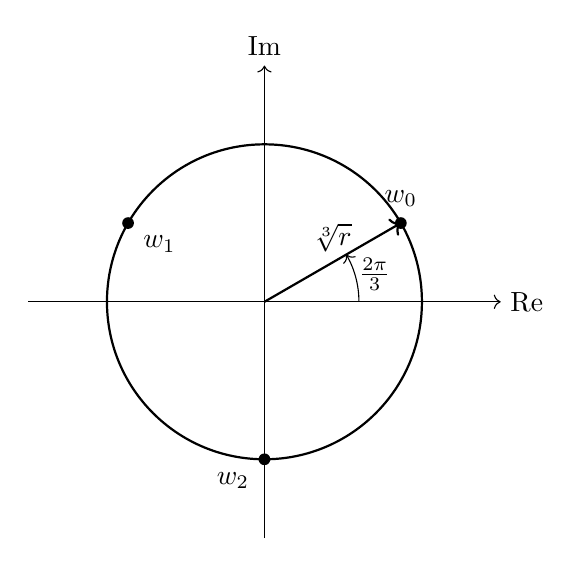
\begin{tikzpicture}

			\draw[->] (-3,0) -- (3,0) node[right] {Re};
			\draw[->] (0,-3) -- (0,3) node[above] {Im};

			% Draw the circle
			\draw[thick] (0,0) circle (2cm);

			% Plot the roots
			\foreach \k in {0, 1, 2} {
					\node[fill,circle,inner sep=1.5pt,label={90-\k*120:$w_\k$}] at ({2*cos(30+\k*120)},{2*sin(30+\k*120)}) {};
				}

			% Draw the radius
			\draw[->,thick] (0,0) -- ({2*cos(30)},{2*sin(30)}) node[midway,above] {\( \sqrt[3]{r} \)};

			% Label the angle
			\draw[->] (1.2,0) arc (0:30:1.2);
			\node at (1.4,0.35) {\( \frac{2\pi}{3} \)};
		\end{tikzpicture}
	\end{center}
}

\chapter{Functions}

\section{Modulus Functions}

\dfn{Modulus function}{

	\begin{center}
		\begin{tikzpicture}
			\begin{axis}[
					xlabel={$x$},
					ylabel={$y$},
					axis lines=middle,
					legend pos=outer north east,
					samples=100,
					domain=-3:3,
					restrict y to domain=-5:5,
					width=10cm, height=8cm,
					xtick={-3,-2,-1,0,1,2,3},
					ytick={-4,-3,-2,-1,0,1,2,3,4},
				]
				% f(x) = x^3 - x
				\addplot [blue, thick] {x^3 - x};
				\addlegendentry{$f(x) = x^3 - x$}

				% |f(x)| = |x^3 - x|
				\addplot [red, thick, dashed] {abs(x^3 - x)};
				\addlegendentry{$|f(x)| = |x^3 - x|$}

				% f(|x|) = |x|^3 - |x|
				\addplot [green, thick, dotted] {abs(x)^3 - abs(x)};
				\addlegendentry{$f(|x|) = |x|^3 - |x|$}
			\end{axis}
		\end{tikzpicture}

	\end{center}

}

\section{Asymptodes}

\dfn{Asymptotes in Rational Functions}{
	Asymptotes are lines that a function approaches as its input approaches a specific value or infinity. They can be horizontal, vertical, or oblique (with a slope).

	\begin{center}
		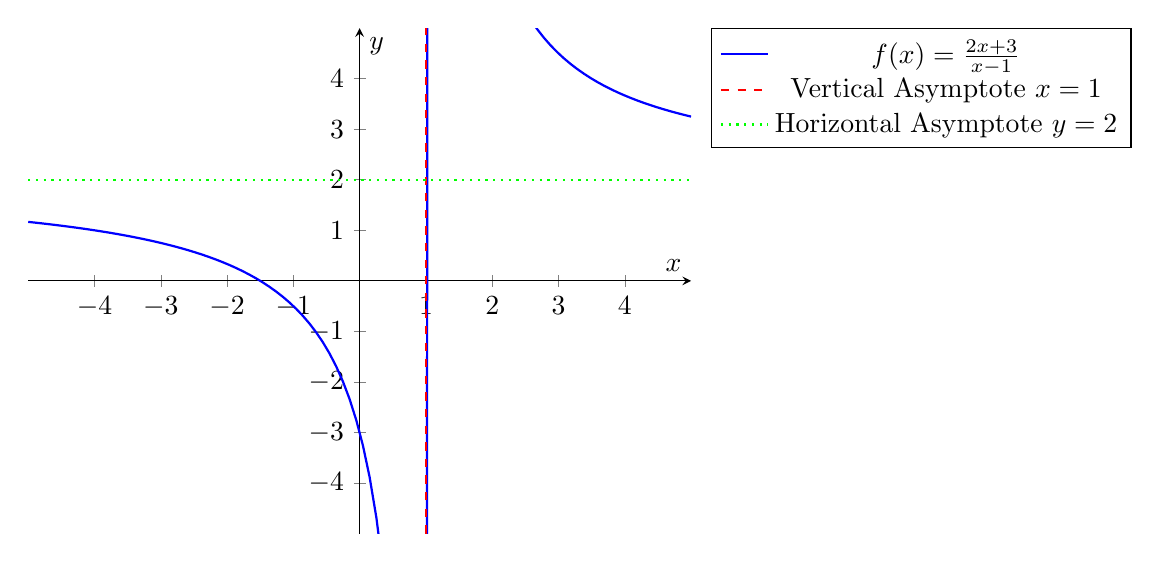
\begin{tikzpicture}
			\begin{axis}[
					xlabel={$x$},
					ylabel={$y$},
					axis lines=middle,
					legend pos=outer north east,
					samples=100,
					domain=-5:5,
					ymin=-5, ymax=5,
					xmin=-5, xmax=5,
					width=10cm, height=8cm,
					xtick={-4,-3,-2,-1,0,1,2,3,4},
					ytick={-4,-3,-2,-1,0,1,2,3,4},
				]
				% Plot the rational function f(x) = (2x+3)/(x-1)
				\addplot [blue, thick] {(2*x + 3)/(x - 1)};
				\addlegendentry{$f(x) = \frac{2x+3}{x-1}$}

				% Plot the vertical asymptote x = 1
				\addplot [red, thick, dashed] coordinates {(1,-5) (1,5)};
				\addlegendentry{Vertical Asymptote $x = 1$}

				% Plot the horizontal asymptote y = 2
				\addplot [green, thick, dotted] coordinates {(-5,2) (5,2)};
				\addlegendentry{Horizontal Asymptote $y = 2$}

			\end{axis}
		\end{tikzpicture}
	\end{center}

	\textbf{For some function}:

	$$f(x) = \frac{ax+b}{cx-d}$$

	\textbf{Vertical asymptote}:

	$$x = \frac{-d}{c}$$

	\textbf{Horizontal asymptote}:

	$$y = \frac{a}{c}$$

}

\dfn{Asymptotes in Division of Polynomials}{
	If the degree of the numerator is greater than the degree of the denominator, there is no horizontal asymptote.


	\begin{center}
		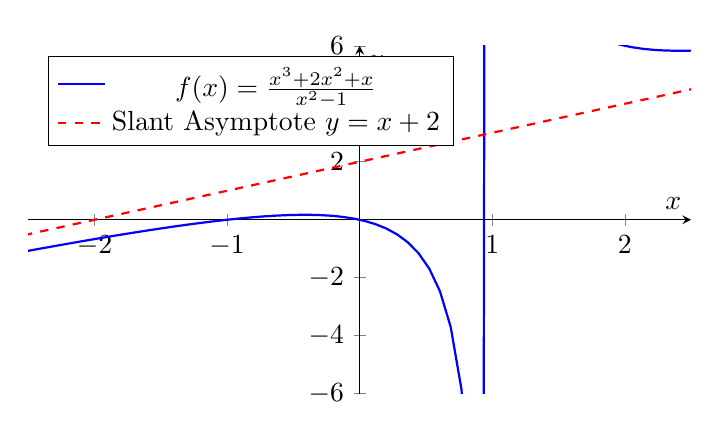
\begin{tikzpicture}
			\begin{axis}[
					xlabel={$x$},
					ylabel={$y$},
					axis lines=middle,
					samples=100,
					domain=-4:4,
					ymin=-6, ymax=6,
					xmin=-2.5, xmax=2.5,
					width=10cm, height=6cm,
					xtick={-2,-1,0,1,2},
					ytick={-6,-4,-2,0,2,4,6},
					legend pos=north west,
				]
				% Plot the rational function f(x) = (x^3 + 2x^2 + x)/(x^2 - 1)
				\addplot [blue, thick] {(x^3 + 2*x^2 + x)/(x^2 - 1)};
				\addlegendentry{$f(x) = \frac{x^3 + 2x^2 + x}{x^2 - 1}$}

				% Optionally, plot the slant asymptote for reference
				\addplot [red, thick, dashed] {x + 2};
				\addlegendentry{Slant Asymptote $y = x + 2$}
			\end{axis}
		\end{tikzpicture}
	\end{center}

	To find the oblique asymptote, do the division of the numerator and denominator polynomials

	If the degree of the numerator is less than the degree of the denominator, the horizontal asymptote is $y=0$

	\begin{center}
		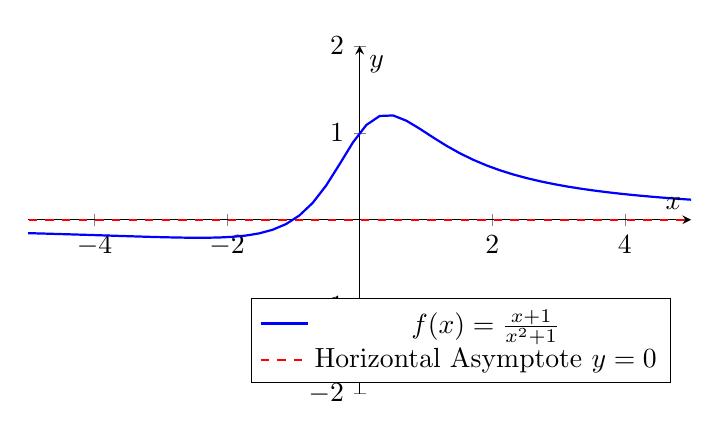
\begin{tikzpicture}
			\begin{axis}[
					xlabel={$x$},
					ylabel={$y$},
					axis lines=middle,
					samples=100,
					domain=-10:10,
					ymin=-2, ymax=2,
					xmin=-5, xmax=5,
					width=10cm, height=6cm,
					xtick={-4,-2,0,2,4},
					ytick={-2,-1,0,1,2},
					legend pos=south east,
				]
				% Plot the rational function f(x) = (x + 1)/(x^2 + 1)
				\addplot [blue, thick] {(x + 1)/(x^2 + 1)};
				\addlegendentry{$f(x) = \frac{x + 1}{x^2 + 1}$}

				% Plot the horizontal asymptote y = 0
				\addplot [red, thick, dashed] {0};
				\addlegendentry{Horizontal Asymptote $y = 0$}

			\end{axis}
		\end{tikzpicture}
	\end{center}


	If the degree of the numerator is equal to the degree of the denominator, do as for rational functions
}

\section{Odd and Even Functions}

\dfn{Even Functions}{
	A function \( f(x) \) is called an \textbf{even function} if it satisfies the condition:
	\[
		f(-x) = f(x) \quad \text{for all } x \text{ in the domain of } f.
	\]
	Geometrically, the graph of an even function is symmetric with respect to the \( y \)-axis.

	\begin{center}
		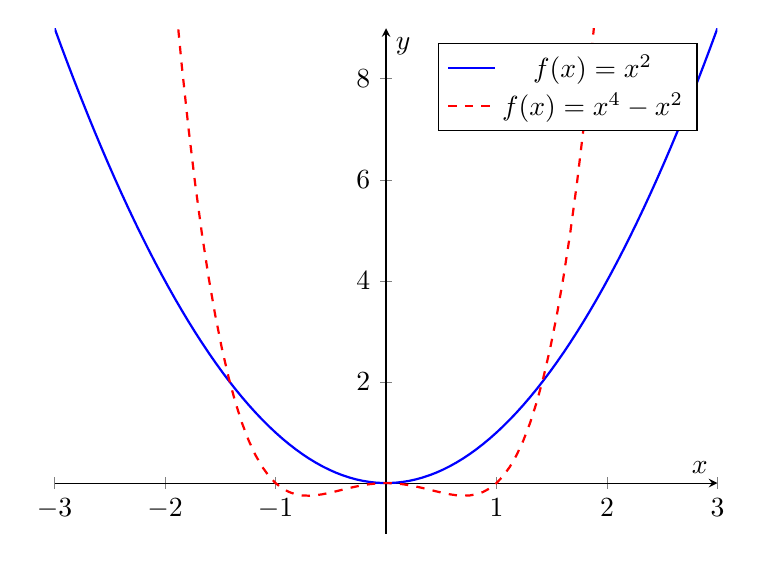
\begin{tikzpicture}
			\begin{axis}[
					xlabel={$x$},
					ylabel={$y$},
					axis lines=middle,
					samples=100,
					domain=-3:3,
					ymin=-1, ymax=9,
					width=10cm, height=8cm,
					xtick={-3,-2,-1,0,1,2,3},
					ytick={0,2,4,6,8},
					legend pos=north east,
				]
				% Plot the even function f(x) = x^2
				\addplot [blue, thick] {x^2};
				\addlegendentry{$f(x) = x^2$}

				% Plot the even function f(x) = x^4 - x^2
				\addplot [red, thick, dashed] {x^4 - x^2};
				\addlegendentry{$f(x) = x^4 - x^2$}
			\end{axis}
		\end{tikzpicture}
	\end{center}
}

\dfn{Odd Functions}{
	A function \( f(x) \) is called an \textbf{odd function} if it satisfies the condition:
	\[
		f(-x) = -f(x) \quad \text{for all } x \text{ in the domain of } f.
	\]
	Geometrically, the graph of an odd function is symmetric with respect to the origin.

	\begin{center}
		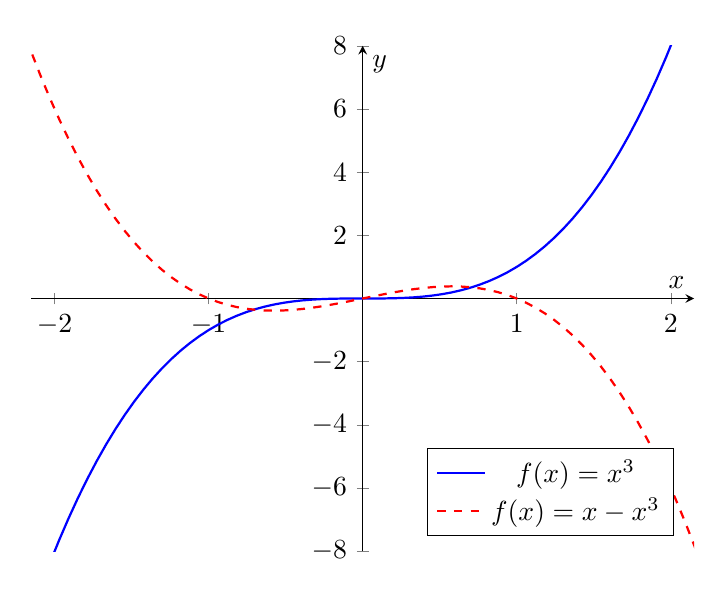
\begin{tikzpicture}
			\begin{axis}[
					xlabel={$x$},
					ylabel={$y$},
					axis lines=middle,
					samples=100,
					domain=-3:3,
					ymin=-8, ymax=8,
					width=10cm, height=8cm,
					xtick={-3,-2,-1,0,1,2,3},
					ytick={-8,-6,-4,-2,0,2,4,6,8},
					legend pos=south east,
				]
				% Plot the odd function f(x) = x^3
				\addplot [blue, thick] {x^3};
				\addlegendentry{$f(x) = x^3$}

				% Plot the odd function f(x) = x - x^3
				\addplot [red, thick, dashed] {x - x^3};
				\addlegendentry{$f(x) = x - x^3$}
			\end{axis}
		\end{tikzpicture}
	\end{center}
}

\section{Reciprocal Functions}

\dfn{Reciprocal Function}{
	A \textbf{reciprocal function} is a function of the form:
	\[
		f(x) = \frac{1}{g(x)}
	\]
	where \( g(x) \) is a non-zero function. The most basic example of a reciprocal function is \( f(x) = \frac{1}{x} \).

	The behavior of a reciprocal function depends heavily on the nature of \( g(x) \):

	\begin{itemize}
		\item \textbf{Zeros of \( g(x) \)}: These correspond to vertical asymptotes in \( f(x) \) because the function becomes undefined at these points.
		\item \textbf{Maxima and Minima of \( g(x) \)}: These correspond to minima and maxima of \( f(x) \), respectively, but with inverted values.
		\item \textbf{Asymptotes}: If \( g(x) \) has a horizontal asymptote, \( f(x) \) will have a horizontal asymptote at the reciprocal of this value.
	\end{itemize}

	\begin{center}
		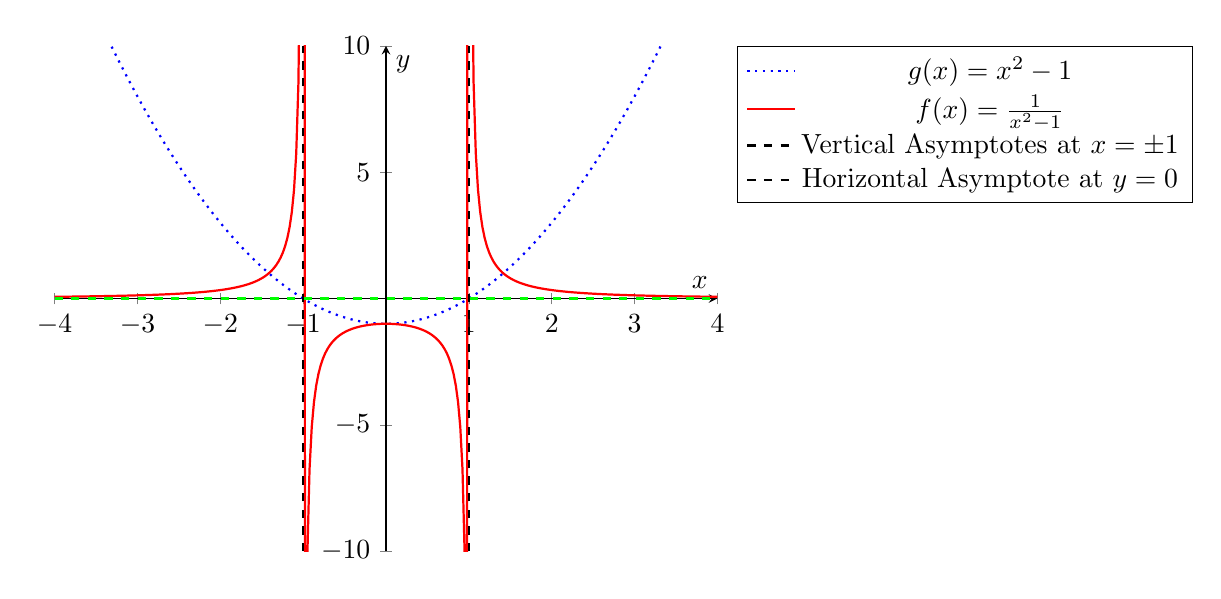
\begin{tikzpicture}
			\begin{axis}[
					xlabel={$x$},
					ylabel={$y$},
					axis lines=middle,
					samples=300,
					domain=-4:4,
					ymin=-10, ymax=10,
					width=10cm, height=8cm,
					xtick={-4,-3,-2,-1,0,1,2,3,4},
					ytick={-10,-5,0,5,10},
					legend pos=outer north east,
					unbounded coords=jump,
				]
				% Plot g(x) = x^2 - 1
				\addplot [blue, thick, dotted] {x^2 - 1};
				\addlegendentry{$g(x) = x^2 - 1$}

				% Plot the reciprocal function f(x) = 1/(x^2 - 1)
				\addplot [red, thick] {1/(x^2 - 1)};
				\addlegendentry{$f(x) = \frac{1}{x^2 - 1}$}

				% Plot vertical asymptotes at x = -1 and x = 1
				\addplot [black, thick, dashed] coordinates {(-1,-10) (-1,10)};
				\addplot [black, thick, dashed] coordinates {(1,-10) (1,10)};
				\addlegendentry{Vertical Asymptotes at $x = \pm 1$}

				% Plot horizontal asymptote at y = 0
				\addplot [green, thick, dashed] coordinates {(-4,0) (4,0)};
				\addlegendentry{Horizontal Asymptote at $y = 0$}
			\end{axis}
		\end{tikzpicture}
	\end{center}
}

\ex{Example of a Reciprocal Function}{
	Consider the reciprocal function:
	\[
		f(x) = \frac{1}{x^2 - 1}
	\]

	Let's analyze its key features:

	\begin{itemize}
		\item \textbf{Zeros of \( g(x) \)}: The zeros of \( g(x) = x^2 - 1 \) are \( x = \pm 1 \). These correspond to vertical asymptotes in \( f(x) \).
		\item \textbf{Minima and Maxima}: The function \( g(x) \) has a minimum at \( x = 0 \), where \( g(0) = -1 \). The reciprocal function \( f(x) \) has a corresponding maximum at \( x = 0 \), where \( f(0) = -1 \).
		\item \textbf{Horizontal Asymptote}: As \( x \) approaches infinity, \( g(x) \) approaches infinity, so \( f(x) \) approaches 0, leading to a horizontal asymptote at \( y = 0 \).
	\end{itemize}
}


\section{Factor and Remainder Theorems}

\dfn{Remainder Theorem}{
	The Remainder Theorem states that if a polynomial $f(x)$ is divided by a linear divisor of the form $x - c$, the remainder of this division is $f(c)$. In other words, to find the remainder when dividing $f(x)$ by $x - c$, simply substitute $c$ into the polynomial.

}

\ex{Using the Remainder Theorem}{
	Consider the polynomial:
	\[
		f(x) = 2x^3 - 3x^2 + 4x - 5
	\]
	We want to find the remainder when $f(x)$ is divided by $x - 2$.

	According to the Remainder Theorem, the remainder is $f(2)$. Substituting $x = 2$ into $f(x)$ gives:
	\[
		f(2) = 2(2)^3 - 3(2)^2 + 4(2) - 5
	\]
	\[
		f(2) = 2(8) - 3(4) + 8 - 5
	\]
	\[
		f(2) = 16 - 12 + 8 - 5 =
	\]
	Thus, the remainder is 7.
}

\dfn{Factor Theorem}{
	The Factor Theorem is a special case of the Remainder Theorem. It states that a polynomial $f(x)$ has a factor $x - c$ if and only if $f(c) = 0$. This means that $c$ is a root (or zero) of the polynomial if and only if $x - c$ is a factor of $f(x)$.
}

\ex{Using the Factor Theorem}{
	Let's check if $x - 3$ is a factor of the polynomial:
	\[
		f(x) = x^3 - 7x + 6
	\]
	According to the Factor Theorem, we need to check whether $f(3) = 0$. Substituting $x = 3$ into $f(x)$ gives:
	\[
		f(3) = (3)^3 - 7(3) + 6
	\]
	\[
		f(3) = 27 - 21 + 6 = 12
	\]
	Since $f(3) \neq 0$, $x - 3$ is not a factor of $f(x)$.

}

\ex{Finding Factors using the Factor Theorem}{

	Now, let's find a factor of the polynomial:
	\[
		g(x) = x^3 - 4x^2 + x + 6
	\]
	We test possible values of $c$ by substituting them into $g(x)$ until we find one that makes $g(c) = 0$.

	First, let's try $x = 2$:
	\[
		g(2) = (2)^3 - 4(2)^2 + 2 + 6
	\]
	\[
		g(2) = 8 - 16 + 2 + 6 = 0
	\]
	Since $g(2) = 0$, $x - 2$ is a factor of $g(x)$.

	Thus, we can factor $g(x)$ as:
	\[
		g(x) = (x - 2)(x^2 - 2x - 3)
	\]
	Further factoring $x^2 - 2x - 3$ gives:
	\[
		g(x) = (x - 2)(x - 3)(x + 1)
	\]
	So, the complete factorization of $g(x)$ is:
	\[
		g(x) = (x - 2)(x - 3)(x + 1)
	\]
}

\section{Sums and Products of Roots of Polynomials}

\dfn{Sums and Products of Roots}{
	For any polynomial of degree \( n \) with real or complex coefficients, given by:
	\[
		P(x) = a_n x^n + a_{n-1} x^{n-1} + \dots + a_1 x + a_0 = 0
	\]
	where \( a_n \neq 0 \), the roots \( r_1, r_2, \dots, r_n \) of the polynomial satisfy certain relationships, which are derived from Vieta's formulas:

	\begin{itemize}
		\item \textbf{Sum of the roots:}
		      \[
			      r_1 + r_2 + \dots + r_n = -\frac{a_{n-1}}{a_n}
		      \]
		\item \textbf{Sum of the products of the roots taken two at a time:}
		      \[
			      r_1r_2 + r_1r_3 + \dots + r_{n-1}r_n = \frac{a_{n-2}}{a_n}
		      \]
		\item \textbf{Product of the roots:}
		      \[
			      r_1r_2 \dots r_n = (-1)^n \frac{a_0}{a_n}
		      \]
	\end{itemize}
}

\ex{Example for a Quadratic Polynomial}{
	Consider the quadratic polynomial:
	\[
		P(x) = ax^2 + bx + c = 0
	\]
	with roots \( r_1 \) and \( r_2 \). According to Vieta's formulas:

	\begin{itemize}
		\item \textbf{Sum of the roots:}
		      \[
			      r_1 + r_2 = -\frac{b}{a}
		      \]
		\item \textbf{Product of the roots:}
		      \[
			      r_1r_2 = \frac{c}{a}
		      \]
	\end{itemize}
}

\ex{Example for a Cubic Polynomial}{
	Consider the cubic polynomial:
	\[
		P(x) = ax^3 + bx^2 + cx + d = 0
	\]
	with roots \( r_1 \), \( r_2 \), and \( r_3 \). According to Vieta's formulas:

	\begin{itemize}
		\item \textbf{Sum of the roots:}
		      \[
			      r_1 + r_2 + r_3 = -\frac{b}{a}
		      \]
		\item \textbf{Sum of the products of the roots taken two at a time:}
		      \[
			      r_1r_2 + r_1r_3 + r_2r_3 = \frac{c}{a}
		      \]
		\item \textbf{Product of the roots:}
		      \[
			      r_1r_2r_3 = -\frac{d}{a}
		      \]
	\end{itemize}
}

\chapter{Vectors and Planes}

\section{Vectors}

\dfn{Vectors}{
	A \textbf{vector} is a mathematical object that has both magnitude and direction. Vectors can be represented in several forms:

	\begin{itemize}
		\item Component Form: A vector \( \mathbf{v} \) in \( \mathbb{R}^n \) can be represented by its components along the coordinate axes. In \( \mathbb{R}^3 \), for example:
		      \[
			      \mathbf{v} = \begin{pmatrix} v_1 \\ v_2 \\ v_3 \end{pmatrix} = v_1 \hat{i} + v_2 \hat{j} + v_3 \hat{k}
		      \]
		      where \( v_1, v_2, v_3 \) are the components, and \( \hat{i}, \hat{j}, \hat{k} \) are the unit vectors along the x, y, and z axes respectively.

		\item Magnitude-Direction Form: A vector \( \mathbf{v} \) can also be represented by its magnitude (length) and direction (unit vector):
		      \[
			      \mathbf{v} = |\mathbf{v}| \hat{v}
		      \]
		      where \( |\mathbf{v}| \) is the magnitude of \( \mathbf{v} \), and \( \hat{v} \) is the unit vector in the direction of \( \mathbf{v} \).

		\item Position Vector: The position vector \( \mathbf{r} \) represents the position of a point \( P(x, y, z) \) in space relative to the origin:
		      \[
			      \mathbf{r} = x \hat{i} + y \hat{j} + z \hat{k} = \begin{pmatrix} x \\ y \\ z \end{pmatrix}
		      \]
	\end{itemize}
}

\dfn{Vector Notation}{
	Vectors are typically denoted by boldface letters, such as \( \mathbf{v} \), \( \mathbf{a} \), or \( \mathbf{b} \), or by letters with an arrow on top, such as \( \vec{v} \). The magnitude (or length) of a vector \( \mathbf{v} \) is denoted by \( |\mathbf{v}| \) or \( \| \mathbf{v} \| \).

	In component form, a vector can be written as:
	\[
		\mathbf{v} = \begin{pmatrix} v_1 \\ v_2 \\ v_3 \end{pmatrix}
	\]
	or \( \mathbf{v} = v_1 \hat{i} + v_2 \hat{j} + v_3 \hat{k} \) in \( \mathbb{R}^3 \).

	\begin{center}
		\begin{tikzpicture}
			% Draw the vector
			\draw[->, thick] (0,0) -- (3,2) node[right] {\( \mathbf{v} \)};
			% Draw the axes
			\draw[->] (-1,0) -- (4,0) node[right] {x};
			\draw[->] (0,-1) -- (0,3) node[above] {y};
			% Components
			\draw[dashed] (3,0) -- (3,2);
			\draw[dashed] (0,2) -- (3,2);
			\node[below] at (3,0) {\( v_1 \)};
			\node[left] at (0,2) {\( v_2 \)};
		\end{tikzpicture}
	\end{center}
}

\section{Planes}

\dfn{Planes}{
	A \textbf{plane} is a flat, two-dimensional surface that extends infinitely in all directions. There are several ways to represent a plane in \( \mathbb{R}^3 \):

	\begin{itemize}
		\item General Form: The general equation of a plane is given by:
		      \[
			      ax + by + cz = d
		      \]
		      where \( a, b, c \) are the coefficients that define the orientation of the plane, and \( d \) is the distance from the origin along the normal vector \( \mathbf{n} = \begin{pmatrix} a \\ b \\ c \end{pmatrix} \).

		\item Point-Normal Form: A plane can also be defined by a point \( P_0(x_0, y_0, z_0) \) on the plane and a normal vector \( \mathbf{n} = \begin{pmatrix} a \\ b \\ c \end{pmatrix} \). The equation of the plane is:
		      \[
			      a(x - x_0) + b(y - y_0) + c(z - z_0) = 0
		      \]

		\item Parametric Form: The plane can be represented parametrically as:
		      \[
			      \mathbf{r}(s, t) = \mathbf{r}_0 + s \mathbf{v}_1 + t \mathbf{v}_2
		      \]
		      where \( \mathbf{r}_0 \) is the position vector of a point on the plane, and \( \mathbf{v}_1, \mathbf{v}_2 \) are direction vectors lying on the plane.

		\item Intercept Form: When a plane intercepts the x, y, and z axes at points \( a, b, c \) respectively, the equation of the plane can be written as:
		      \[
			      \frac{x}{a} + \frac{y}{b} + \frac{z}{c} = 1
		      \]

		\item **Vector-Normal Form**: The equation of a plane can be expressed using the dot product between the position vector \( \mathbf{r} = \begin{pmatrix} x \\ y \\ z \end{pmatrix} \) and the normal vector \( \mathbf{n} = \begin{pmatrix} a \\ b \\ c \end{pmatrix} \). The equation is:
		      \[
			      \mathbf{r} \cdot \mathbf{n} = \mathbf{a} \cdot \mathbf{n}
		      \]
		      where \( \mathbf{a} = \begin{pmatrix} x_0 \\ y_0 \\ z_0 \end{pmatrix} \) is a known point on the plane.

	\end{itemize}
}

\begin{center}
	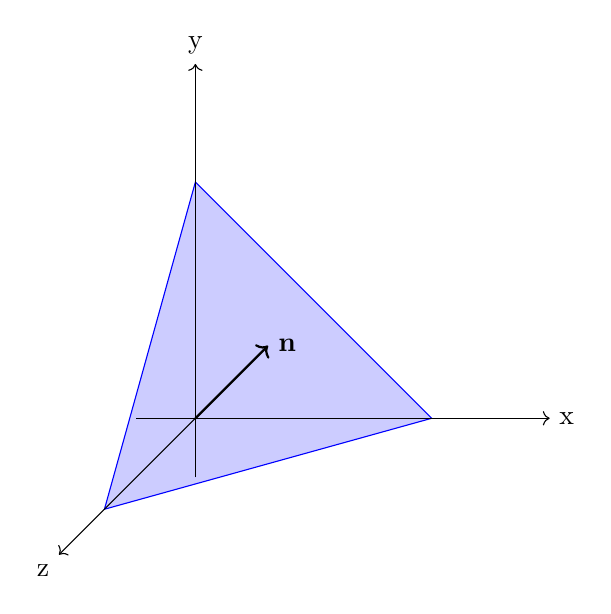
\begin{tikzpicture}[scale=1.5]
		% Draw the plane
		\filldraw[fill=blue!20, draw=blue] (2,0,0) -- (0,2,0) -- (0,0,2) -- cycle;
		% Draw the normal vector
		\draw[->, thick] (0,0,0) -- (1,1,1) node[right] {\( \mathbf{n} \)};
		% Draw the axes
		\draw[->] (-0.5,0,0) -- (3,0,0) node[right] {x};
		\draw[->] (0,-0.5,0) -- (0,3,0) node[above] {y};
		\draw[->] (0,0,-0.5) -- (0,0,3) node[below left] {z};
	\end{tikzpicture}
\end{center}s

\section{Operations with Vectors}

\dfn{Scalar Product (Dot Product)}{
	The \textbf{scalar product} (or \textbf{dot product}) of two vectors \( \mathbf{a} \) and \( \mathbf{b} \) in \( \mathbb{R}^n \) is defined as:
	\[
		\mathbf{a} \cdot \mathbf{b} = a_1b_1 + a_2b_2 + \dots + a_nb_n
	\]
	In \( \mathbb{R}^3 \), for vectors \( \mathbf{a} = \begin{pmatrix} a_1 \\ a_2 \\ a_3 \end{pmatrix} \) and \( \mathbf{b} = \begin{pmatrix} b_1 \\ b_2 \\ b_3 \end{pmatrix} \), the dot product is:
	\[
		\mathbf{a} \cdot \mathbf{b} = a_1b_1 + a_2b_2 + a_3b_3
	\]
	The dot product can also be expressed in terms of the magnitudes of \( \mathbf{a} \) and \( \mathbf{b} \) and the angle \( \theta \) between them:
	\[
		\mathbf{a} \cdot \mathbf{b} = |\mathbf{a}| |\mathbf{b}| \cos \theta
	\]
	The dot product is a scalar quantity and is zero when the vectors are orthogonal (perpendicular).
}

\dfn{Vector Product (Cross Product)}{
	The \textbf{vector product} (or \textbf{cross product}) of two vectors \( \mathbf{a} \) and \( \mathbf{b} \) in \( \mathbb{R}^3 \) is a vector \( \mathbf{c} \) that is perpendicular to both \( \mathbf{a} \) and \( \mathbf{b} \), and its magnitude is given by:
	\[
		|\mathbf{c}| = |\mathbf{a} \times \mathbf{b}| = |\mathbf{a}| |\mathbf{b}| \sin \theta
	\]
	where \( \theta \) is the angle between \( \mathbf{a} \) and \( \mathbf{b} \). The cross product is calculated as:
	\[
		\mathbf{a} \times \mathbf{b} = \begin{vmatrix}
			\hat{i} & \hat{j} & \hat{k} \\
			a_1     & a_2     & a_3     \\
			b_1     & b_2     & b_3
		\end{vmatrix} = (a_2b_3 - a_3b_2)\hat{i} - (a_1b_3 - a_3b_1)\hat{j} + (a_1b_2 - a_2b_1)\hat{k}
	\]
	The result of a cross product is a vector perpendicular to the plane formed by \( \mathbf{a} \) and \( \mathbf{b} \), with a direction given by the right-hand rule.
}

\dfn{Angle Between Two Vectors}{
	The angle \( \theta \) between two vectors \( \mathbf{a} \) and \( \mathbf{b} \) can be found using the dot product:
	\[
		\cos \theta = \frac{\mathbf{a} \cdot \mathbf{b}}{|\mathbf{a}| |\mathbf{b}|}
	\]
	Solving for \( \theta \):
	\[
		\theta = \cos^{-1} \left( \frac{\mathbf{a} \cdot \mathbf{b}}{|\mathbf{a}| |\mathbf{b}|} \right)
	\]
	This formula is valid for any non-zero vectors \( \mathbf{a} \) and \( \mathbf{b} \).
}

\ex{Example: Dot Product and Cross Product}{
Consider the vectors \( \mathbf{a} = \begin{pmatrix} 2 \\ -1 \\ 3 \end{pmatrix} \) and \( \mathbf{b} = \begin{pmatrix} 1 \\ 4 \\ -2 \end{pmatrix} \).

\textbf{Dot Product:}
\[
	\mathbf{a} \cdot \mathbf{b} = 2(1) + (-1)(4) + 3(-2) = 2 - 4 - 6 = -8
\]

\textbf{Cross Product:}
\[
\mathbf{a} \times \mathbf{b} = \begin{vmatrix}
	\hat{i} & \hat{j} & \hat{k} \\
	2       & -1      & 3       \\
	1       & 4       & -2
\end{vmatrix} = \hat{i}(-1 \times -2 - 3 \times 4) - \hat{j}(2 \times -2 - 3 \times 1) + \hat{k}(2 \times 4 - (-1) \times 1)
\]
\[
\mathbf{a} \times \mathbf{b} = \hat{i}(2 - 12) - \hat{j}(-4 - 3) + \hat{k}(8 + 1) = -10\hat{i} + 7\hat{j} + 9\hat{k}
\]

\textbf{Angle Between \( \mathbf{a} \) and \( \mathbf{b} \):}
\[
|\mathbf{a}| = \sqrt{2^2 + (-1)^2 + 3^2} = \sqrt{4 + 1 + 9} = \sqrt{14}
\]
\[
|\mathbf{b}| = \sqrt{1^2 + 4^2 + (-2)^2} = \sqrt{1 + 16 + 4} = \sqrt{21}
\]
\[
\cos \theta = \frac{-8}{\sqrt{14} \times \sqrt{21}}
\]
Thus, the angle \( \theta \) is:
\[
\theta = \cos^{-1} \left( \frac{-8}{\sqrt{14 \times 21}} \right)
\]
}

\dfn{Graphical Representations}{

	\textbf{Dot Product:}
	\begin{center}
		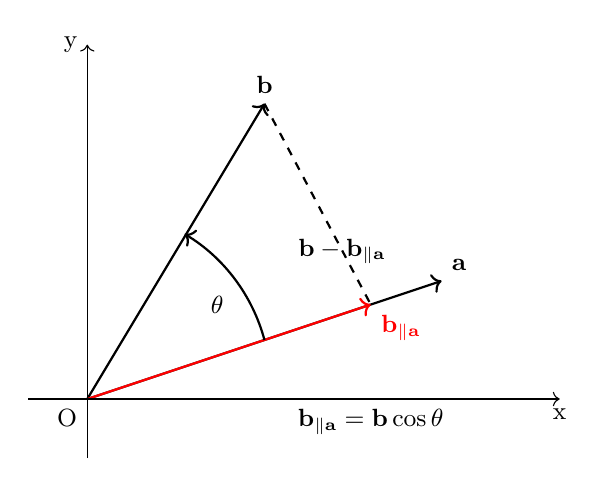
\begin{tikzpicture}[scale=1.5, thick, font=\small]

			% Draw the vectors a and b
			\draw[->, thick] (0,0) -- (3,1) node[above right] {\(\mathbf{a}\)};
			\draw[->, thick] (0,0) -- (1.5,2.5) node[above] {\(\mathbf{b}\)};

			% Projection of b onto a
			\draw[dashed, thick] (1.5,2.5) -- (2.4,0.8);
			\draw[->, thick, red] (0,0) -- (2.4,0.8) node[below right] {\(\mathbf{b}_{\parallel \mathbf{a}}\)};

			% Draw the angle theta
			\draw[->] (1.5,0.5) arc[start angle=15,end angle=59,radius=1.5];
			\node at (1.1,0.8) {\(\theta\)};

			% Labels and additional elements
			\node[below] at (2.4,0) {\(\mathbf{b}_{\parallel \mathbf{a}} = \mathbf{b} \cos \theta\)};
			\node[right] at (1.7,1.25) {\(\mathbf{b} - \mathbf{b}_{\parallel \mathbf{a}}\)};

			% Draw the axes
			\draw[->, thin] (-0.5,0) -- (4,0) node[below] {x};
			\draw[->, thin] (0,-0.5) -- (0,3) node[left] {y};

			% Draw the origin
			\node[below left] at (0,0) {O};

		\end{tikzpicture}
	\end{center}

	\textbf{Cross Product:}
	\begin{center}
		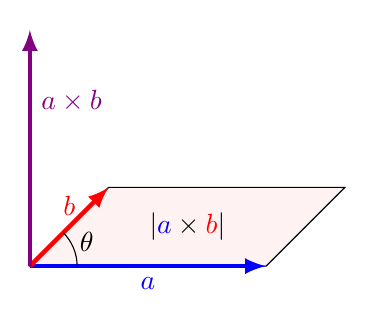
\begin{tikzpicture}
			\draw[-,fill=white!95!red](0,0)--(3,0)--(4,1)--(1,1)--cycle;
			\node at (2,0.5) {$|\textcolor{blue}{a}\times \textcolor{red}{b}|$};
			\draw[ultra thick,-latex,blue](0,0)--(3,0)node[midway,below]{$a$};
			\draw[ultra thick,-latex,red](0,0)--(1,1)node[midway,above]{$b$};
			\draw[ultra thick,-latex,blue!50!red](0,0)--(0,3)node[pos=0.7,right]{$a\times b$};
			\draw (0.6,0) arc [start angle=0,end angle=45,radius=0.6]
			node[pos=0.7,right]{$\theta$};
		\end{tikzpicture}
	\end{center}

}

\section{Distances in Geometry}

\dfn{Distance Between Two Lines}{
	The distance between two skew lines (lines that do not intersect and are not parallel) in \( \mathbb{R}^3 \) can be found using the following method:

	Consider two lines given by their parametric equations:
	\[
		\mathbf{r}_1(t) = \mathbf{r}_0 + t\mathbf{a}, \quad \mathbf{r}_2(s) = \mathbf{r}_0' + s\mathbf{b}
	\]
	where \( \mathbf{r}_0 \) and \( \mathbf{r}_0' \) are points on the respective lines, and \( \mathbf{a} \) and \( \mathbf{b} \) are direction vectors of the lines.

	The distance \( d \) between the two lines is given by:
	\[
		d = \frac{|(\mathbf{r}_0' - \mathbf{r}_0) \cdot (\mathbf{a} \times \mathbf{b})|}{|\mathbf{a} \times \mathbf{b}|}
	\]
	where \( \mathbf{a} \times \mathbf{b} \) is the cross product of the direction vectors of the two lines, and \( \mathbf{r}_0' - \mathbf{r}_0 \) is the vector connecting points on the two lines.

	If the lines are parallel, \( \mathbf{a} \times \mathbf{b} = \mathbf{0} \), and the formula is not applicable. In this case, the distance is the distance between any point on one line to the other line.
}

\dfn{Distance Between a Point and a Line}{
	The distance \( d \) from a point \( \mathbf{P}_0(x_0, y_0, z_0) \) to a line defined by a point \( \mathbf{P}_1(x_1, y_1, z_1) \) and a direction vector \( \mathbf{d} = \begin{pmatrix} a \\ b \\ c \end{pmatrix} \) is given by:
	\[
		d = \frac{|\mathbf{d} \times (\mathbf{P}_0 - \mathbf{P}_1)|}{|\mathbf{d}|}
	\]
	where \( \mathbf{P}_0 - \mathbf{P}_1 = \begin{pmatrix} x_0 - x_1 \\ y_0 - y_1 \\ z_0 - z_1 \end{pmatrix} \) is the vector from the point on the line to the point \( \mathbf{P}_0 \), and \( \mathbf{d} \times (\mathbf{P}_0 - \mathbf{P}_1) \) is the cross product of \( \mathbf{d} \) and \( \mathbf{P}_0 - \mathbf{P}_1 \).

	Alternatively, the distance can be expressed as:
	\[
		d = \frac{|a(x_0 - x_1) + b(y_0 - y_1) + c(z_0 - z_1)|}{\sqrt{a^2 + b^2 + c^2}}
	\]
}

\dfn{Distance Between a Point and a Plane}{
	The distance \( d \) from a point \( \mathbf{P}_0(x_0, y_0, z_0) \) to a plane given by the equation \( ax + by + cz + d = 0 \) is:
	\[
		d = \frac{|ax_0 + by_0 + cz_0 + d|}{\sqrt{a^2 + b^2 + c^2}}
	\]
	This formula gives the perpendicular distance from the point to the plane.
}

\ex{Example: Distance Between a Point and a Plane}{
	Consider the point \( \mathbf{P}_0(1, 2, 3) \) and the plane given by the equation \( 2x - y + 2z - 4 = 0 \).

	The distance \( d \) from the point to the plane is calculated as follows:
	\[
		d = \frac{|2(1) - 1(2) + 2(3) - 4|}{\sqrt{2^2 + (-1)^2 + 2^2}} = \frac{|2 - 2 + 6 - 4|}{\sqrt{4 + 1 + 4}} = \frac{2}{\sqrt{9}} = \frac{2}{3}
	\]

	Therefore, the distance from the point \( \mathbf{P}_0(1, 2, 3) \) to the plane \( 2x - y + 2z - 4 = 0 \) is \( \frac{2}{3} \).
}

\section{Graphical Representations (BAD)}

\dfn{Distance Between Two Lines (Skew Lines)}{
	\begin{center}
		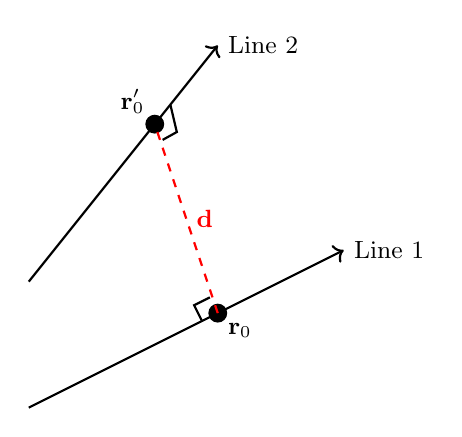
\begin{tikzpicture}[scale=2, thick, font=\small]

			% Draw the first line
			\draw[->, thick] (-1,-1) -- (1,0) node[right] {Line 1};


			% Draw the second line
			\draw[->, thick] (-1,-0.2) -- (0.2,1.3) node[right] {Line 2};

			% Draw points on the lines
			\filldraw[black] (0.2,-0.4) circle (1.5pt) node[below right] {\(\mathbf{r}_0\)};
			\filldraw[black] (-0.2,0.8) circle (1.5pt) node[above left] {\(\mathbf{r}_0'\)};

			% Draw the connecting vector (shortest distance)
			\draw[dashed, thick, red] (0.2,-0.4) -- (-0.2,0.8) node[midway, right] {\(\mathbf{d}\)};

			% Indicate the perpendicularity
			\draw[thick] (-0.15,0.70) -- (-0.06,0.75) -- (-0.1,0.92);
			\draw[thick] (0.15,-0.3) -- (0.05,-0.35) -- (0.1,-0.45);

		\end{tikzpicture}
	\end{center}
}

\dfn{Distance Between a Point and a Line}{
	\begin{center}
		\begin{tikzpicture}[scale=1.5, thick, font=\small]

			% Draw the line
			\draw[->, thick] (-2,-1) -- (2,1) node[right] {Line};

			% Draw the point
			\filldraw[black] (1.5,2.5) circle (1.5pt) node[above right] {Point \( \mathbf{P}_0 \)};

			% Draw point on the line
			\filldraw[black] (0,0) circle (1.5pt) node[below left] {\( \mathbf{P}_1 \)};

			% Draw the perpendicular from the point to the line
			\draw[dashed, thick, red] (1.5,2.5) -- (0,0) node[midway, right] {Distance \( d \)};
		\end{tikzpicture}
	\end{center}

}

\dfn{Distance Between a Point and a Plane}{

	\begin{center}
		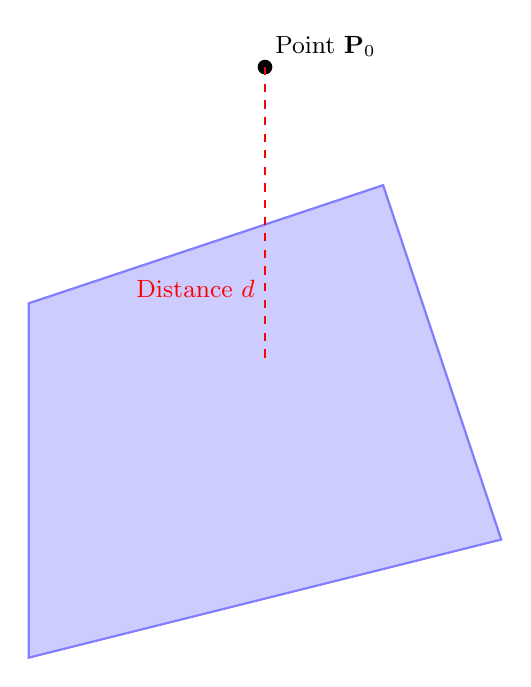
\begin{tikzpicture}[scale=1.5, thick, font=\small]

			% Draw the plane
			\filldraw[fill=blue!20, draw=blue!50] (-2,-2) -- (2,-1) -- (1,2) -- (-2,1) -- cycle;

			% Draw the point
			\filldraw[black] (0,3) circle (1.5pt) node[above right] {Point \( \mathbf{P}_0 \)};

			% Draw the perpendicular from the point to the plane
			\draw[dashed, thick, red] (0,3) -- (0,0.5) node[near end, left] {Distance \( d \)};
		\end{tikzpicture}
	\end{center}
}

\section{Intersections between planes}

\dfn{Intersection Between two planes}{
	The intersection between two planes is always a line which lies in both planes. Its vector equation can be found by computing the vector product of the normal vector of the planes.


	\begin{center}
		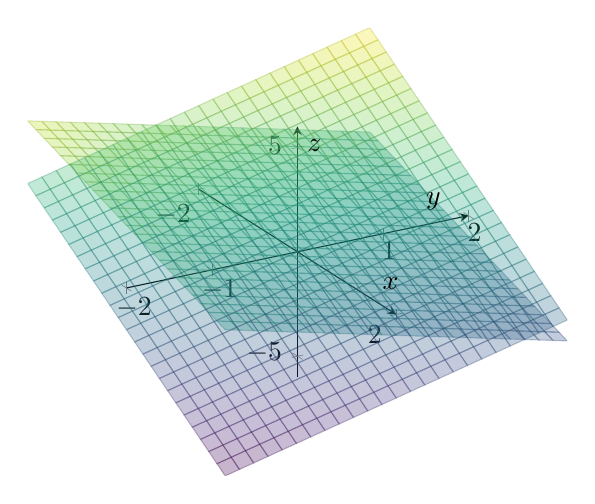
\begin{tikzpicture}
			\begin{axis}[
					view={60}{30}, % Adjust the viewing angle
					axis lines=center,
					xlabel={$x$},
					ylabel={$y$},
					zlabel={$z$},
					colormap/viridis, % Color map for the planes
				]

				% First plane: x + y + z = 1
				\addplot3[surf, opacity=0.3, domain=-2:2, y domain=-2:2]
				{1 - x - y};

				% Second plane: 2x - y + z = 0
				\addplot3[surf, opacity=0.3, domain=-2:2, y domain=-2:2]
				{y - 2*x};

			\end{axis}
		\end{tikzpicture}
	\end{center}
}

\dfn{Intersection Between Three Planes}{
	The intersection between three planes is always a point which lies of all three planes. Its vector equation can be found by computing the vector product of the normal vector of the planes, or all pairs of lines which are intersections between the pairs of planes.
	\begin{center}
		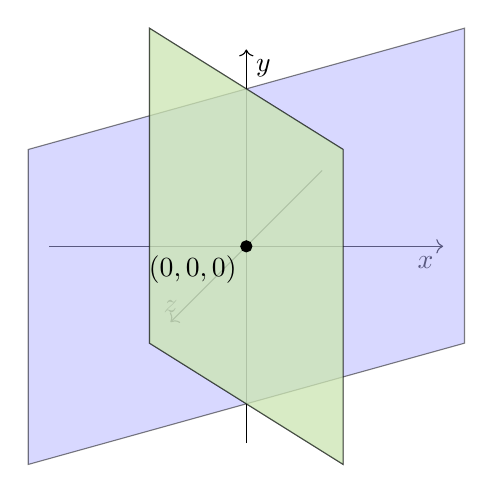
\begin{tikzpicture}

			\draw[->] (-2.5,0,0) -- (2.5,0,0) node[anchor=north east] {$x$};
			\draw[->] (0,-2.5,0) -- (0,2.5,0) node[anchor=north west] {$y$};
			\draw[->] (0,0,-2.5) -- (0,0,2.5) node[anchor=south] {$z$};

			% Define the planes
			\filldraw[fill=blue!30, opacity=0.5] (2,-2,-2) -- (2,2,-2) -- (-2,2,2) -- (-2,-2,2) -- cycle;
			\filldraw[fill=red!30, opacity=0.5] (2,-2,2) -- (2,2,2) -- (-2,2,-2) -- (-2,-2,-2) -- cycle;
			\filldraw[fill=green!30, opacity=0.5] (-2,-2,-2) -- (-2,2,-2) -- (2,2,2) -- (2,-2,2) -- cycle;

			% Add the intersection point
			\filldraw[black] (0,0,0) circle (2pt) node[anchor=north east] {$(0,0,0)$};

		\end{tikzpicture}
	\end{center}

}

\end{document}